%% =============================================================
%%  Preprint — Compact Single-Column Style
%% =============================================================
\documentclass[10pt,a4paper]{article}

%% ---------- page geometry ----------
\usepackage[top=2.0cm, bottom=2.0cm, left=2.0cm, right=2.0cm]{geometry}
\setlength{\parskip}{2pt plus 1pt minus 1pt}  % compact inter-paragraph spacing

%% ---------- fonts & encoding ----------
\usepackage[utf8]{inputenc}
\usepackage[T1]{fontenc}
\usepackage[protrusion=true,expansion=false]{microtype}  % improved typography
%% ---------- math ----------
\usepackage{amsmath,amssymb,amsfonts,mathtools}
\usepackage{amsthm}
\IfFileExists{newtxtext.sty}{%
  \usepackage{newtxtext,newtxmath}  % Times-like fonts (arXiv standard)
}{}
\newtheorem{proposition}{Proposition}

%% ---------- tables ----------
\usepackage{booktabs}
\IfFileExists{multirow.sty}{\usepackage{multirow}}{}
\providecommand{\multirow}[3]{#3}
\usepackage{tabularx}
\usepackage{array}
\usepackage{colortbl}
\IfFileExists{makecell.sty}{\usepackage{makecell}}{}
\providecommand{\makecell}[2][]{\begin{tabular}{@{}c@{}}#2\end{tabular}}

%% ---------- figures ----------
\usepackage{graphicx}
\usepackage{subcaption}
\usepackage[font={footnotesize,it},labelfont={bf,up},labelsep=period,
            justification=justified,singlelinecheck=false,
            margin=0.5cm]{caption}
\usepackage{float}
\IfFileExists{placeins.sty}{%
  \usepackage{placeins}            % float barrier support (manual only)
}{%
  \providecommand{\FloatBarrier}{}
}
\IfFileExists{needspace.sty}{%
  \usepackage{needspace}
}{%
  \newcommand{\Needspace}[1]{%
    \par\begingroup
    \dimen0=##1\relax
    \ifdim\pagegoal<\maxdimen
      \ifdim\dimexpr\pagegoal-\pagetotal\relax<\dimen0
        \break
      \fi
    \fi
    \endgroup}
}
\IfFileExists{standalone.sty}{\usepackage{standalone}}{}

%% ---------- float placement (prevent figures drifting to end) ----------
\renewcommand{\topfraction}{0.9}          % max fraction of page for floats at top
\renewcommand{\bottomfraction}{0.8}       % max fraction of page for floats at bottom
\renewcommand{\textfraction}{0.1}         % min fraction of page for text
\renewcommand{\floatpagefraction}{0.8}    % min fraction for a float-only page
\setcounter{topnumber}{4}                 % max floats at top of page
\setcounter{bottomnumber}{4}              % max floats at bottom of page
\setcounter{totalnumber}{8}               % max floats per page total

%% ---------- tighter float spacing (reduce white space around figures) ----------
\setlength{\textfloatsep}{6pt plus 2pt minus 2pt}   % space between float and text
\setlength{\floatsep}{4pt plus 2pt minus 1pt}       % space between two floats
\setlength{\intextsep}{6pt plus 2pt minus 2pt}      % space around in-text floats
\setlength{\dblfloatsep}{6pt plus 2pt minus 2pt}    % space for double-column floats
\setlength{\abovecaptionskip}{4pt}                   % space above caption
\setlength{\belowcaptionskip}{0pt}                   % space below caption

\setlength{\abovedisplayskip}{6pt plus 2pt minus 2pt}
\setlength{\belowdisplayskip}{6pt plus 2pt minus 2pt}
\setlength{\abovedisplayshortskip}{2pt plus 2pt minus 1pt}
\setlength{\belowdisplayshortskip}{2pt plus 2pt minus 1pt}

%% ---------- typography ----------
\widowpenalty=10000
\clubpenalty=10000
\usepackage{array}
\setlength{\extrarowheight}{1pt}

%% ---------- formatting ----------
\usepackage[authoryear,round]{natbib}
\IfFileExists{cleveref.sty}{%
  \usepackage[capitalize]{cleveref}
  \crefname{figure}{Fig.}{Figs.}
  \Crefname{figure}{Fig.}{Figs.}
  \crefname{table}{Table}{Tables}
  \Crefname{table}{Table}{Tables}
  \crefname{section}{Section}{Sections}
  \Crefname{section}{Section}{Sections}
}{%
  \providecommand{\cref}[1]{\ref{##1}}
  \providecommand{\Cref}[1]{\ref{##1}}
  \providecommand{\crefrange}[2]{\ref{##1}--\ref{##2}}
  \providecommand{\Crefrange}[2]{\ref{##1}--\ref{##2}}
}
\usepackage[dvipsnames]{xcolor}
% Colors for TikZ Figure 1
\definecolor{navy}{HTML}{1b2a4a}
\definecolor{teal}{HTML}{1a7a6d}
\definecolor{dteal}{HTML}{0d4f47}
\definecolor{lgrey}{HTML}{f0f2f5}
\definecolor{mgrey}{HTML}{b0b8c4}
\definecolor{rmcol}{HTML}{9ca3af}
\definecolor{faccol}{HTML}{2d9d8f}
\definecolor{distcol}{HTML}{3b82c4}
\definecolor{retcol}{HTML}{e06060}
\definecolor{shadowcol}{HTML}{d0d4da}
\IfFileExists{enumitem.sty}{%
  \usepackage{enumitem}
  \setlist{noitemsep,topsep=2pt,parsep=0pt,partopsep=0pt}
}{%
  \let\origitemize\itemize
  \let\endorigitemize\enditemize
  \renewenvironment{itemize}[1][]{\origitemize}{\endorigitemize}
  \let\origenumerate\enumerate
  \let\endorigenumerate\endenumerate
  \renewenvironment{enumerate}[1][]{\origenumerate}{\endorigenumerate}
}
\usepackage{fancyhdr}
\IfFileExists{abstract.sty}{%
  \usepackage{abstract}
}{%
  \newcommand{\abstractnamefont}{}
  \newlength{\absleftindent}
  \newlength{\absrightindent}
}
\IfFileExists{titlesec.sty}{\usepackage{titlesec}}{}

%% ---------- code / monospace ----------
\PassOptionsToPackage{hyphens}{url}
\usepackage{url}

%% ---------- hyperlink styling ----------
\usepackage{hyperref}
\hypersetup{
  colorlinks  = true,
  linkcolor   = NavyBlue,
  citecolor   = OliveGreen,
  urlcolor    = BrickRed,
  pdfauthor   = {Reza Barati, Qinmin Vivian Hu},
  pdftitle    = {Supplementary Material for gym-invmgmt: An Open Benchmarking Framework for Inventory Management Methods},
  pdfsubject  = {Inventory Management, Reinforcement Learning, Operations Research},
  pdfkeywords = {RL, benchmark, supply chain, GNN, stochastic programming}
}
\usepackage{bookmark}

%% ---------- preprint header ----------
\pagestyle{fancy}
\fancyhf{}
\fancyhead[L]{\small\textit{Supplementary Material}}
\fancyhead[R]{\small\textit{\today}}
\fancyfoot[C]{\thepage}
\renewcommand{\headrulewidth}{0pt}

%% ---------- compact section styling ----------
\IfFileExists{titlesec.sty}{%
  \titleformat{\section}{\large\bfseries}{\thesection}{1em}{}
  \titleformat{\subsection}{\normalsize\bfseries}{\thesubsection}{1em}{}
  \titlespacing*{\section}{0pt}{1.2ex plus 0.3ex minus .2ex}{0.6ex plus .2ex}
  \titlespacing*{\subsection}{0pt}{0.8ex plus 0.2ex minus .2ex}{0.4ex plus .2ex}
}{}

%% ---------- abstract styling ----------
\renewcommand{\abstractnamefont}{\normalfont\bfseries}
\setlength{\absleftindent}{1.0cm}
\setlength{\absrightindent}{1.0cm}

%% ---------- short-hands ----------
\newcommand{\ie}{\textit{i.e.}}
\newcommand{\eg}{\textit{e.g.}}
\newcommand{\etal}{\textit{et~al.}}
\newcommand{\cf}{\textit{cf.}}
\newcommand{\RR}{\mathbb{R}}
\usepackage{pifont}
\newcommand{\cmark}{\ding{51}}
\newcommand{\xmark}{\ding{55}}

%% ---------- table row coloring ----------
\definecolor{lightgray}{gray}{0.93}
\definecolor{tableheader}{HTML}{2C3E50}
\definecolor{tableaccent}{HTML}{E8F4FD}
\definecolor{headerblue}{HTML}{1A5276}


%% =============================================================
%%  SUPPLEMENTARY FRONT MATTER
%% =============================================================
\begin{document}

\title{\textbf{Supplementary Material for\\[4pt]
       gym-invmgmt: An Open Benchmarking Framework\\[4pt]
       for Inventory Management Methods}}

\author{%
  Reza Barati\thanks{Corresponding author:
  \texttt{r2barati@torontomu.ca}}
  \quad Qinmin Vivian Hu\\[4pt]
  \small Department of Computer Science\\[-1pt]
  \small Toronto Metropolitan University, Toronto, ON, Canada
}

\date{%
  \small\today\\[4pt]
  \small\textcolor{gray}{Supplementary material.}%
}

\maketitle
\thispagestyle{fancy}

\noindent
This document provides supplementary tables, figures, diagnostics, and
implementation details for the manuscript
\emph{gym-invmgmt: An Open Benchmarking Framework for Inventory Management
Methods}. It is intended to accompany the main manuscript during submission
and peer review.

\setcounter{table}{0}
\setcounter{figure}{0}
\renewcommand{\thetable}{S\arabic{table}}
\renewcommand{\thefigure}{S\arabic{figure}}

%% ================================================================
%%  APPENDIX
%% ================================================================
\appendix
\setlength{\parskip}{1pt plus 0.5pt minus 0.5pt}
\makeatletter
\renewcommand\section{\@startsection{section}{1}{\z@}%
  {1.0ex plus .2ex minus .2ex}{0.6ex plus .1ex}%
  {\normalfont\Large\bfseries}}
% Appendix floats are intentionally allowed to float.  Forcing every appendix
% table/figure with [H] or flushing floats before each section creates large
% blank regions whenever a tall object barely misses the remaining page space.
\let\appendix@section\section
\renewcommand{\section}[1]{\Needspace{3\baselineskip}\appendix@section{#1}}
\renewcommand\subsection{\@startsection{subsection}{2}{\z@}%
  {0.8ex plus .2ex minus .2ex}{0.45ex plus .1ex}%
  {\normalfont\large\bfseries}}
\renewcommand\paragraph{\@startsection{paragraph}{4}{\z@}%
  {0.45ex plus .1ex minus .1ex}{-0.65em}%
  {\normalfont\normalsize\bfseries}}
\makeatother
%% ================================================================
%%  APPENDIX A — Complete Scenario Enumeration
%% ================================================================
\section{Complete Scenario Enumeration}\label{app:scenarios}

Rows~1--22 in \Cref{tab:full_scenarios} enumerate the core scenarios used
for the main benchmark aggregates; rows~23--26 enumerate the supplemental
MARL-mode rows included in the merged 26-scenario artifact but excluded
from the 22-scenario core aggregate. The conceptual full factorial
($2 \times 4 \times 2 \times 2 = 32$) is reduced because stationary
and M5 external-trace profiles are not paired with endogenous goodwill, and the
M5 external trace is evaluated only under backlog fulfillment. Scenario
IDs abbreviate topology (B=default/base, S=serial), demand profile
(St, M5, TS, TSS), goodwill (G/NG), and fulfillment mode (BL/LS);
exact keys and factor columns are stored in the released CSV.
The M5 rows use a real 30-day item-store sales window from
\texttt{sales\_train\_evaluation}: \texttt{FOODS\_3\_382} at store
\texttt{CA\_3}, days \texttt{d\_1841}--\texttt{d\_1870}. The raw path
has mean 16.03, coefficient of variation 1.37, and nonzero sales on
83.3\% of days; scaling by $20/16.03$ matches the benchmark demand scale
while preserving its empirical temporal shape. These rows do not use
\texttt{calendar.csv} or \texttt{sell\_prices.csv}; costs, lead times,
and capacities are those of the benchmark topology. Thus M5 contributes
an empirical terminal-demand path, not an observed Walmart replenishment
network.

\begin{table}[!tbp]
\centering
\caption{Complete enumeration of the 26-scenario merged artifact. Rows~1--22
form the core evaluation grid; rows~23--26 are supplemental MARL-mode rows.}
\label{tab:full_scenarios}
\label{tab:supplemental_marl_scenarios}
\scriptsize
\renewcommand{\arraystretch}{1.06}
\begin{tabular}{@{} c l l c c l @{}}
\toprule
\textbf{\#}
  & \textbf{Network}
  & \textbf{Demand Profile}
  & \textbf{Goodwill}
  & \textbf{Fulfill.}
  & \textbf{Scenario ID} \\
\midrule
\rowcolor{lightgray}
1  & Default (9-node) & Stationary          & Off & BL & B-St-NG-BL  \\
2  & Default          & Stationary          & Off & LS & B-St-NG-LS  \\
\rowcolor{lightgray}
3  & Default          & M5-derived volatile & Off & BL & B-M5-NG-BL  \\
4  & Default          & Trend+Seasonal      & Off & BL & B-TS-NG-BL  \\
\rowcolor{lightgray}
5  & Default          & Trend+Seasonal      & Off & LS & B-TS-NG-LS  \\
6  & Default          & Trend+Seas.+Shock   & Off & BL & B-TSS-NG-BL \\
\rowcolor{lightgray}
7  & Default          & Trend+Seas.+Shock   & Off & LS & B-TSS-NG-LS \\
8  & Default          & Trend+Seasonal      & On  & BL & B-TS-G-BL   \\
\rowcolor{lightgray}
9  & Default          & Trend+Seasonal      & On  & LS & B-TS-G-LS   \\
10 & Default          & Trend+Seas.+Shock   & On  & BL & B-TSS-G-BL  \\
\rowcolor{lightgray}
11 & Default          & Trend+Seas.+Shock   & On  & LS & B-TSS-G-LS  \\
\midrule
12 & Serial (5-node)  & Stationary          & Off & BL & S-St-NG-BL  \\
\rowcolor{lightgray}
13 & Serial           & Stationary          & Off & LS & S-St-NG-LS  \\
14 & Serial           & M5-derived volatile & Off & BL & S-M5-NG-BL  \\
\rowcolor{lightgray}
15 & Serial           & Trend+Seasonal      & Off & BL & S-TS-NG-BL  \\
16 & Serial           & Trend+Seasonal      & Off & LS & S-TS-NG-LS  \\
\rowcolor{lightgray}
17 & Serial           & Trend+Seas.+Shock   & Off & BL & S-TSS-NG-BL \\
18 & Serial           & Trend+Seas.+Shock   & Off & LS & S-TSS-NG-LS \\
\rowcolor{lightgray}
19 & Serial           & Trend+Seasonal      & On  & BL & S-TS-G-BL   \\
20 & Serial           & Trend+Seasonal      & On  & LS & S-TS-G-LS   \\
\rowcolor{lightgray}
21 & Serial           & Trend+Seas.+Shock   & On  & BL & S-TSS-G-BL  \\
22 & Serial           & Trend+Seas.+Shock   & On  & LS & S-TSS-G-LS  \\
\midrule
\multicolumn{6}{@{}l}{\textit{Supplemental MARL-mode rows, excluded from the 22-scenario core aggregate}} \\
\rowcolor{lightgray}
23 & Default (9-node) & Trend+Seasonal      & Off & BL & B-TS-NG-BL-MARL  \\
24 & Default          & Trend+Seas.+Shock   & Off & BL & B-TSS-NG-BL-MARL \\
\rowcolor{lightgray}
25 & Serial (5-node)  & Trend+Seasonal      & Off & BL & S-TS-NG-BL-MARL  \\
26 & Serial           & Trend+Seas.+Shock   & Off & BL & S-TSS-NG-BL-MARL \\
\bottomrule
\end{tabular}
\end{table}

%% ================================================================
%%  APPENDIX B — Mathematical Notation
%% ================================================================
\section{Mathematical Notation}\label{sec:appendix_notation}

\Cref{tab:notation} summarizes the mathematical notation used
throughout the paper for the multi-echelon supply chain formulation.

\begin{table}[!tbp]
\centering
\caption[Mathematical notation for the multi-echelon supply chain.]{%
  Mathematical notation for the multi-echelon supply chain network.}
\label{tab:notation}
\footnotesize
\renewcommand{\arraystretch}{0.98}
\begin{tabularx}{\linewidth}{@{} >{$}c<{$} X @{}}
\toprule
\textbf{Symbol} & \textbf{Definition} \\
\midrule
G = (V, E) & Directed acyclic graph of the supply network \\
V,\; E & Node set and edge set of $G$ \\
E_r \subseteq E & Reorder (upstream) edges; defines the action space \\
M \subseteq V & Managed nodes (excluding raw-material and market nodes) \\
\operatorname{pred}(j),\;\operatorname{succ}(j) & Predecessor / successor nodes of $j$ in $G$ \\
t \in \{1,\dots,T\} & Discrete time period ($T = 30$ in all experiments) \\
X_t^{(j)} & On-hand inventory at node $j$, end of period $t$ \\
a_t^{(e)} & Requested replenishment order (policy action) on edge $e$ at period $t$ \\
R_t^{(e)} & Feasible filled replenishment order on edge $e$ at period $t$ \\
S_t^{(j,k)} & Shipments fulfilled from $j$ to $k$ during period $t$ \\
D_{t} & External customer demand at retailer, period $t$ \\
U_t^{(j,k)} & Unfulfilled demand on retail link $(j,k)$, end of $t$; carried forward only in backlog mode \\
Y_t^{(e)} & In-transit pipeline inventory on edge $e$ at period $t$ \\
L_{ij} & Lead time (periods) between nodes $i$ and $j$ \\
v_j & Production yield factor at factory $j$ \\
C_j & Maximum production capacity at factory $j$ \\
I_0^{(j)} & Initial inventory at node $j$ \\
p_{ij} & Unit transfer price on edge $(i,j)$ \\
h_j & Holding cost per unit per period at node $j$ \\
g_{ij} & Pipeline holding cost per unit per period on edge $(i,j)$ \\
b_{jk} & Backlog/lost-sales penalty per unit on retail link $(j,k)$ \\
o_j & Operating cost coefficient at factory $j$ \\
K_{ij} & Fixed ordering cost on edge $(i,j)$ \\
r_t & Total network reward at period $t$ \\
P_t^{(j)} & Realized profit for managed node $j$ at period $t$ \\
\alpha & Financial profit-discount factor used in the reward equation \\
s_t & Customer goodwill sentiment at period $t$ \\
\lambda_t & Demand mean at period $t$ (Poisson parameter) \\
\bottomrule
\end{tabularx}
\end{table}

%% ================================================================
%%  APPENDIX C — Network Node Parameters
%% ================================================================
\section{Network Node Parameters}\label{sec:appendix_network_params}

\Cref{tab:network_params} reports the exact network parameters used in all
experiments, extracted directly from the \texttt{gym-invmgmt} YAML
configuration files. The grouped layout reduces whitespace while preserving
the original subtable labels used elsewhere in the manuscript.

\begin{table}[!tbp]
\centering
\caption[Network topology parameters.]{Network topology parameters for the
default divergent and serial supply chains. $L$~=~lead time (periods),
$p$~=~transfer price, $g$~=~pipeline holding cost, and $b$~=~shortage
penalty on retail-demand edges.}
\label{tab:network_params}
\scriptsize
\renewcommand{\arraystretch}{1.03}
\setlength{\tabcolsep}{3pt}
\begin{subtable}[t]{0.39\textwidth}
\centering
\caption{Divergent nodes.}
\label{tab:divergent_nodes}
\begin{tabular}{@{} l c c c c c @{}}
\toprule
\textbf{Node} & \textbf{ID} & $I_0$ & $h$ & $C$ & $v$ \\
\midrule
Market  & 0 & --- & ---   & --- & --- \\
Retailer & 1 & 100 & 0.030 & --- & --- \\
Dist.~1 & 2 & 110 & 0.020 & --- & --- \\
Dist.~2 & 3 & 80  & 0.015 & --- & --- \\
Factory~1 & 4 & 400 & 0.012 & 90 & 1.00 \\
Factory~2 & 5 & 350 & 0.013 & 90 & 1.00 \\
Factory~3 & 6 & 380 & 0.011 & 80 & 1.00 \\
Raw~1 & 7 & --- & --- & --- & --- \\
Raw~2 & 8 & --- & --- & --- & --- \\
\bottomrule
\end{tabular}
\end{subtable}
\hfill
\begin{subtable}[t]{0.58\textwidth}
\centering
\caption{Divergent edges.}
\label{tab:divergent_edges}
\begin{tabular}{@{} l c c c c @{}}
\toprule
\textbf{Edge} & $L$ & $p$ & $g$ & $b$ \\
\midrule
Retailer $\to$ Market & --- & 2.000 & ---   & 0.100 \\
Dist.~1 $\to$ Retailer & 5  & 1.500 & 0.010 & --- \\
Dist.~2 $\to$ Retailer & 3  & 1.600 & 0.015 & --- \\
Factory~1 $\to$ Dist.~1 & 8  & 1.000 & 0.008 & --- \\
Factory~1 $\to$ Dist.~2 & 10 & 0.800 & 0.006 & --- \\
Factory~2 $\to$ Dist.~1 & 9  & 0.700 & 0.005 & --- \\
Factory~3 $\to$ Dist.~1 & 11 & 0.750 & 0.007 & --- \\
Factory~3 $\to$ Dist.~2 & 12 & 0.800 & 0.004 & --- \\
Raw~1 $\to$ Factory~1 & 0  & 0.150 & 0.000 & --- \\
Raw~1 $\to$ Factory~2 & 1  & 0.050 & 0.005 & --- \\
Raw~2 $\to$ Factory~2 & 2  & 0.070 & 0.002 & --- \\
Raw~2 $\to$ Factory~3 & 0  & 0.200 & 0.000 & --- \\
\bottomrule
\end{tabular}
\end{subtable}

\vspace{0.35em}
\begin{subtable}[t]{0.39\textwidth}
\centering
\caption{Serial nodes.}
\label{tab:serial_nodes}
\begin{tabular}{@{} l c c c c c @{}}
\toprule
\textbf{Node} & \textbf{ID} & $I_0$ & $h$ & $C$ & $v$ \\
\midrule
Market & 0 & --- & ---   & --- & --- \\
Retailer & 1 & 100 & 0.030 & --- & --- \\
Distributor & 2 & 100 & 0.020 & --- & --- \\
Factory & 3 & 200 & 0.010 & 100 & 1.00 \\
Raw Mat. & 4 & --- & --- & --- & --- \\
\bottomrule
\end{tabular}
\end{subtable}
\hfill
\begin{subtable}[t]{0.58\textwidth}
\centering
\caption{Serial edges.}
\label{tab:serial_edges}
\begin{tabular}{@{} l c c c c @{}}
\toprule
\textbf{Edge} & $L$ & $p$ & $g$ & $b$ \\
\midrule
Retailer $\to$ Market & --- & 2.000 & ---   & 0.100 \\
Distributor $\to$ Retailer & 4  & 1.500 & 0.010 & --- \\
Factory $\to$ Distributor & 4  & 1.000 & 0.005 & --- \\
Raw Mat. $\to$ Factory & 0  & 0.500 & 0.000 & --- \\
\bottomrule
\end{tabular}
\end{subtable}
\end{table}

%% ================================================================
%%  APPENDIX D — Demand Profile Gallery
%% ================================================================
\section{Demand Profile Gallery}\label{sec:appendix_demand}

A central design goal of \texttt{gym-invmgmt} is \emph{composable}
non-stationarity: rather than hard-coding a fixed demand process,
the environment exposes four orthogonal perturbation primitives that
can be combined multiplicatively at initialization time.
This section documents each primitive and its parameterization,
which together generate the synthetic trend, seasonality, shock, and
goodwill portions of the scenario grid in \Cref{app:scenarios}. The M5
rows use an external empirical trace and are documented separately
below.

\paragraph{Stationary baseline.}
The default demand process is $D_t \sim \text{Poisson}(\mu_0)$ with
$\mu_0 = 20$. This serves as the replication baseline for comparison
with prior benchmarks~(ORL, OR-Gym) that assume stationary demand.

\paragraph{Linear trend.}
A monotonic drift is applied via $\mu_t = \mu_0 (1 + \beta t)$ with
$\beta = 0.05$, producing a 150\% increase over the 30-period horizon.
This tests whether agents can track a persistent shift in the demand
mean---a capability that myopic heuristics (Newsvendor, $(s,S)$)
structurally lack because they estimate moments from a sliding window
that lags the true trend.

\paragraph{Sinusoidal seasonality.}
Periodic fluctuations are modeled as
$\mu_t = \mu_0 (1 + A \sin(2\pi t / P))$ with amplitude $A = 0.5$
and period $P = 30$. The full cycle within one episode forces agents
to anticipate both the upswing (requiring pre-positioning of inventory)
and the downswing (requiring restraint to avoid excess holding costs).

\paragraph{Demand shock.}
A step-function disruption doubles the mean at a fixed mid-horizon onset:
$\mu_t = 2\mu_0$ for $t \geq t_{\text{shock}}$, where $t_{\text{shock}} = 15$.
This models sudden market events (e.g., viral demand spikes)
and is the single most discriminating primitive in our benchmark:
as reported in the main benchmark results, the optimality gap between Oracle
and blind MSSP widens from 8\% under stationary demand to 31\% in
the no-goodwill shock rows.

\paragraph{External M5 trace.}
The M5-derived rows do not sample from a parametric distribution.
Instead, they replay the scaled \texttt{FOODS\_3\_382\_CA\_3}
item-store path documented in \Cref{app:scenarios}. The trace is
deterministic within an episode (\texttt{noise\_scale}=0) so the
benchmark measures policy response to an empirical volatile demand path
rather than adding a second layer of synthetic sampling noise. This
mapping uses M5 as an external terminal-demand source. The released data
adapter also supports hierarchy-inferred M5-style topology construction,
but those inferred graphs should be read as planning or aggregation DAGs,
not as physical Walmart distribution networks unless external logistics
data are supplied.

\Cref{fig:demand_gallery} visualizes all four profiles.
Shaded bands denote $\pm 1\sigma$ variance across 30 evaluation
episodes, confirming that the Poisson sampling noise is modest
relative to the systematic non-stationary signal.

\begin{figure}[!htbp]
  \centering
  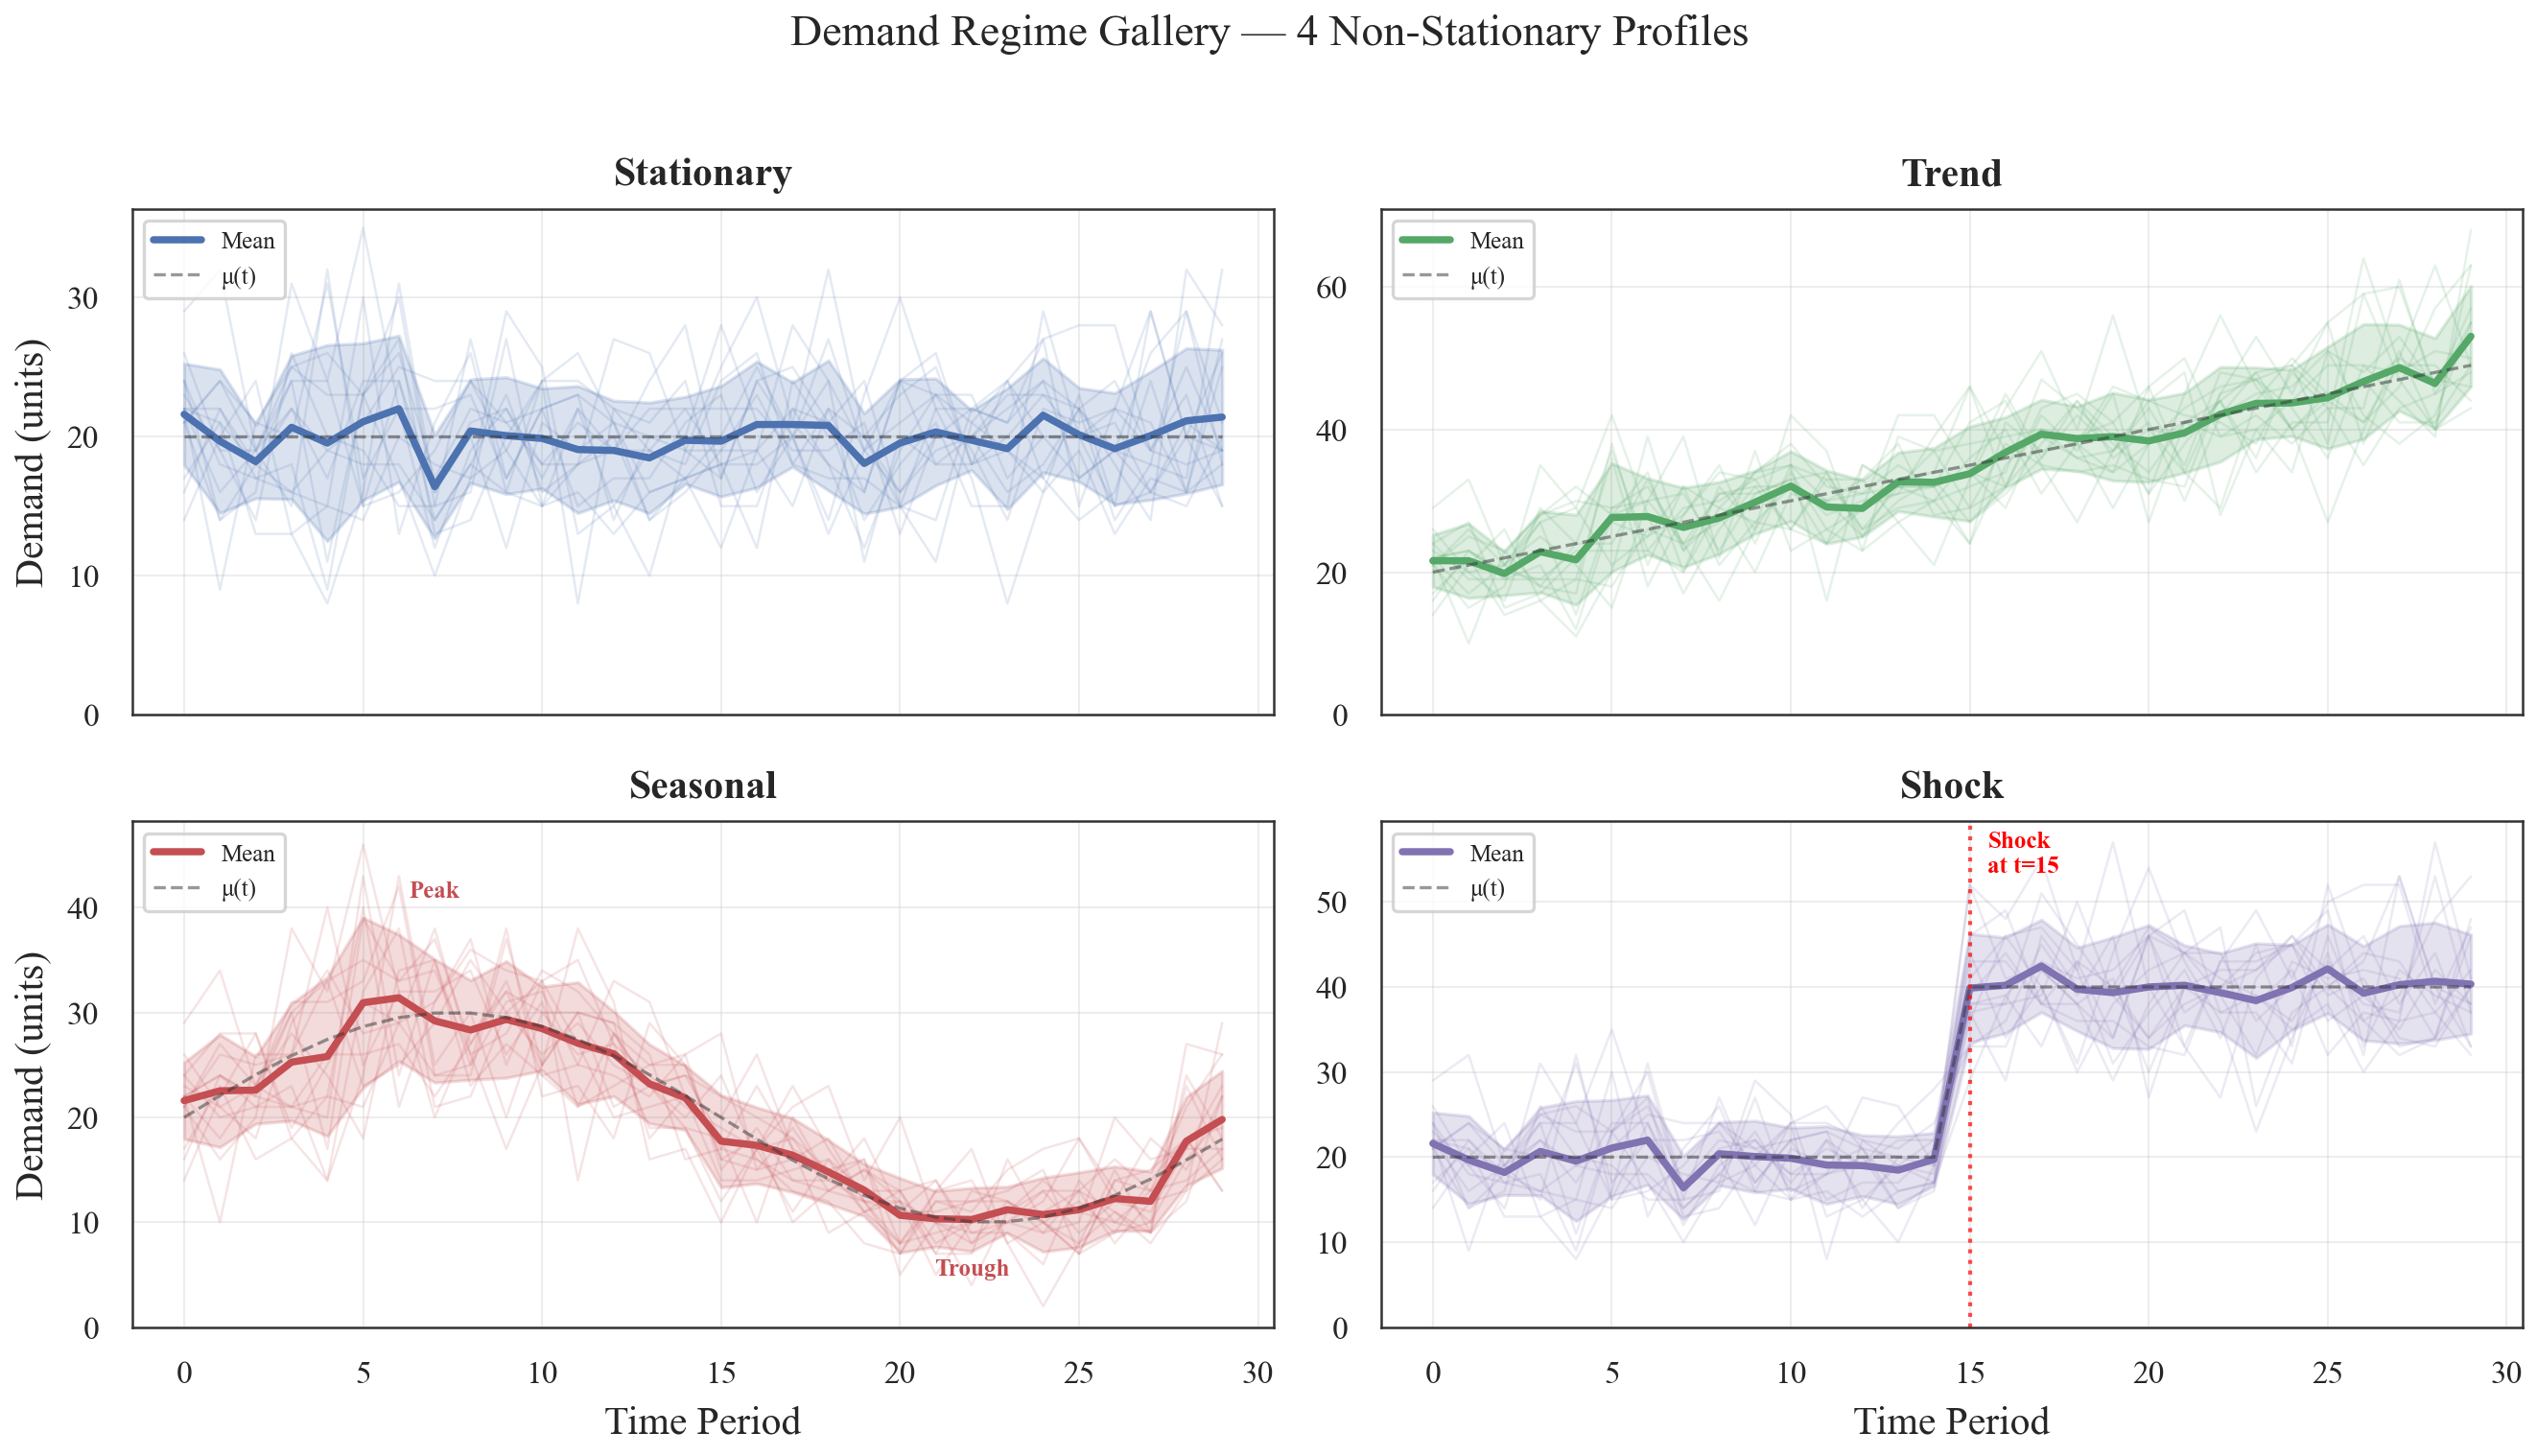
\includegraphics[width=0.82\linewidth]{figures/E1_demand_profile_gallery.png}
  \caption[Non-stationary demand profiles used in the benchmark.]{%
    Composable non-stationary demand profiles.
    \emph{Top-left:} stationary baseline ($\mu = 20$).
    \emph{Top-right:} linear trend ($\mu_t = \mu_0 (1 + 0.05t)$).
    \emph{Bottom-left:} sinusoidal seasonality
    ($\mu_t = \mu_0 (1 + 0.5 \sin(2\pi t / 30))$).
    \emph{Bottom-right:} step-function demand shock
    ($\mu_t = 2\mu_0$ for $t \geq 15$).
    Shaded bands show $\pm 1\sigma$ over 30 evaluation episodes.}
  \label{fig:demand_gallery}
\end{figure}

%% ================================================================
%%  APPENDIX E — Hyperparameters and Neural Architectures
%% ================================================================
\section{Hyperparameters and Neural Architectures}\label{sec:appendix_hyperparams}

\Cref{tab:ppo_hyperparams} lists the shared PPO hyperparameters used by
the main generalist PPO training scripts (PPO-MLP, PPO-GNN,
PPO-Transformer, ST-PPO, and Residual). \Cref{tab:arch_specs} details
the architecture-specific configurations. SAC and imitation-learning
checkpoints use separate serialized optimizer settings reported below.
All RL agents are implemented in Stable-Baselines3~\citep{raffin2021}
with PyTorch~\citep{paszke2019}; the purpose of this appendix is to make
the released evaluation contract reproducible, not to claim an
exhaustive hyperparameter search.

\paragraph{Observation pipeline.}
The raw environment observation is 71~dimensions for the base topology
and 15~for serial. The SB3-based neural checkpoints---PPO-MLP,
PPO-GNN, PPO-Transformer, SAC, GNN-IL, and DAgger---use
\texttt{DomainFeatureWrapper}, which appends normalised
inventory ratios, demand moving averages, pipeline-to-demand ratios,
time-of-horizon features, and goodwill state, producing a
129-dimensional (base) or 49-dimensional (serial) augmented vector.
ST-PPO applies a 4-frame temporal stack to this vector, yielding 516
dimensions for base and 196 for serial. Residual uses the separate
\texttt{PerLinkFeatureWrapper}: 14 features per reorder link, or
154~dimensions for base and 42 for serial. These SB3-based learned
agents use a \texttt{VecNormalize} wrapper with frozen evaluation statistics and
observation clipping at~10.

\paragraph{Action pipeline.}
The environment's native action space is
$\mathcal{A} = [0, a_{\max}]^{n}$.
For PPO-MLP, PPO-GNN, PPO-Transformer, ST-PPO, SAC, GNN-IL, and
DAgger, \texttt{RescaleAction} maps this to $[-1,1]^n$ during training,
and the inverse mapping is applied at evaluation time. Residual instead
predicts a proportional correction to a Newsvendor base action,
$a_t=\operatorname{clip}(a_t^{\mathrm{base}}\odot(1+\delta_t),0,a_{\max})$,
with $\delta_t\in[-0.5,0.5]^n$.

\paragraph{Training budget.}
PPO-MLP is trained for 500{,}000 timesteps; PPO-GNN,
PPO-Transformer, ST-PPO, Residual, and SAC are trained for
200{,}000 timesteps per topology/blindness setting. GNN-IL uses
behavioral cloning followed by 150{,}000 PPO fine-tuning steps, and
DAgger checkpoints are imitation-trained graph policies loaded with
their serialized PPO settings.

\paragraph{Evaluation protocol.}
Each trained checkpoint is evaluated on the full 26-scenario merged
matrix across 10~canonical seeds (260~episodes per agent). The main
text also reports the 22-scenario core grid separately from the four
supplemental MARL-mode scenarios. During evaluation:
(i)~\texttt{VecNormalize} statistics are \emph{frozen}
(\texttt{training=False}), preventing distribution drift;
(ii)~reward normalisation is disabled to ensure raw-reward comparability;
(iii)~actions are selected via \texttt{deterministic=True}
(no stochastic exploration); and
(iv)~the benchmark loads the registry checkpoint together with its
matching saved \texttt{VecNormalize} state. For the generalist PPO, SAC,
Transformer, and Residual training scripts, this deployed checkpoint is
the final policy paired with final normalization statistics; the
\texttt{EvalCallback} logs held-out stationary rewards and diagnostic
best-evaluation artifacts rather than serving as a cross-scenario
model-selection rule.

% --- PPO Hyperparameters + Architecture Specs (side-by-side with subcaptions) ---
\begin{table}[!tbp]
\caption[PPO hyperparameters and architecture specifications.]{%
  Training configuration for the main online RL agents. SAC and
  imitation-learning checkpoints use their own serialized optimizer
  settings described in the text.}
\label{tab:rl_config}
\scriptsize
\renewcommand{\arraystretch}{1.08}
\centering
\begin{subtable}[t]{0.40\textwidth}
\centering
\caption{Shared PPO hyperparameters.}
\label{tab:ppo_hyperparams}
\begin{tabular}{@{} l r @{}}
\toprule
\textbf{Parameter} & \textbf{Value} \\
\midrule
Learning rate       & $3 \times 10^{-4}$ \\
Rollout length      & 2{,}048 \\
Minibatch size      & 512 \\
PPO epochs          & 10 \\
Discount ($\gamma$) & 0.995 \\
GAE $\lambda$       & 0.95 \\
Clip range ($\epsilon$) & 0.2 \\
Entropy coeff.      & 0.005 \\
Value coeff.        & 0.5 \\
Max grad norm       & 0.5 \\
Target KL           & 0.03 \\
\bottomrule
\end{tabular}
\end{subtable}
\hfill
\begin{subtable}[t]{0.56\textwidth}
\centering
\caption{Architecture specifications.}
\label{tab:arch_specs}
\begin{tabular}{@{} l l @{}}
\toprule
\textbf{Agent} & \textbf{Architecture} \\
\midrule
PPO-MLP  & MLP $[256, 128]$ \\
PPO-GNN  & Directed MPNN ($h{=}64$, $L{=}3$, \\
         & bidir., edge-cond.) $\to [256, 128]$ \\
PPO-Transformer & Transformer ($d{=}64$, \\
         & $H{=}4$, $L{=}3$) $\to [256, 128]$ \\
ST-PPO   & Temporal Transformer ($d{=}64$, \\
         & $H{=}4$, $L{=}3$, $n_h{=}4$) $\to [256, 128]$ \\
SAC      & MLP $[256, 256]$ \\
Residual & SharedMLP ($h{=}64$) \\
         & $\to [128, 64]$ \\
GNN-IL   & GNN-V3 BC pretrain $\to$ PPO fine-tune \\
DAgger-G/B & GNN-V3 imitation policy \\
\bottomrule
\end{tabular}
\end{subtable}
\end{table}

\paragraph{Per-architecture training notes.}
\textbf{PPO-MLP} uses a flat two-layer MLP policy ($[256, 128]$, Tanh)
with 133{,}911 trainable parameters (base topology). It is trained for
500{,}000 timesteps to ensure convergence of the larger network, and is
deployed as the saved registry checkpoint paired with its final
normalization statistics. PPO-MLP serves as the flat-policy ablation
baseline: it shows what PPO can achieve \emph{without} graph or temporal
inductive bias.
\textbf{PPO-GNN} replaces the MLP feature extractor with a directed
edge-conditioned MPNN (3~message-passing layers, 64-dim hidden,
attention-weighted aggregation, residual connections, LayerNorm,
BatchNorm), projecting graph-level features to a $[256, 128]$ head.
\textbf{PPO-Transformer} treats each supply-chain node as a token
($d{=}64$), applies 3~self-attention layers ($H{=}4$ heads), and
projects the CLS-pooled output to a $[256, 128]$ policy head.
It is spatial only: the token sequence contains 3~serial nodes or
6~base-topology nodes, with demand history provided as global context
rather than as separate temporal tokens.
\textbf{ST-PPO} extends PPO-Transformer by stacking $n_h{=}4$
temporal frames, creating $(\text{node} \times \text{timestep})$
tokens for joint spatio-temporal attention (12~tokens on serial,
24~tokens on the base topology).
\textbf{SAC} uses Soft Actor-Critic with a flat MLP ($[256, 256]$),
learning rate $3{\times}10^{-4}$, batch size 256, $\gamma=0.99$,
$\tau=0.005$, and automatic entropy tuning.
\textbf{Residual} adds a learned PPO correction to a base-stock
heuristic via \texttt{SharedMLP}~($h{=}64$, $\to [128, 64]$).
\textbf{GNN-IL} uses 50{,}000 Oracle-labeled transitions for GNN-V3
behavioral cloning, followed by 150{,}000 PPO fine-tuning steps with
batch size 64, $\gamma=0.99$, and zero entropy coefficient.
\textbf{DAgger-G/B} are graph imitation policies with
GNN-V3 features, learning rate $10^{-4}$, batch size 64,
$\gamma=0.99$, and zero entropy coefficient.

\Cref{fig:training_curves} shows the evaluation reward during
training for the two primary RL architectures.

\subsection{Development Ablations and Errata}%
\label{sec:ablations}

During development we encountered several implementation pitfalls
whose resolution materially changed the reported results. We document
them here for transparency and to assist future reproducibility
efforts.

\paragraph{A1: PPO-MLP mismatch.}
The initial PPO-MLP checkpoint used the default Stable-Baselines3
network ($[64, 64]$) rather than the intended $[256, 128]$.
With a 129-dimensional augmented observation, the first layer
($129 \to 64$) created a severe information bottleneck, discarding
feature combinations before the policy could form useful representations.
The result was catastrophic:

\begin{center}
\small
\begin{tabular}{@{} l l r r @{}}
\toprule
\textbf{PPO-MLP Variant} & \textbf{Architecture} & \textbf{Mean \$} & \textbf{\% Oracle} \\
\midrule
V2 features, blind     & $[64, 64]$, 200K steps   & $-134$  & $-15.7$ \\
V2 features, blind     & $[256, 128]$, 500K steps & $+873$  & $57.9$  \\
\bottomrule
\end{tabular}
\end{center}

\noindent
\textbf{Root cause:} No explicit \texttt{policy\_kwargs} was passed to
\texttt{PPO()}, so SB3 used its default two-layer $[64, 64]$ Tanh MLP.
\textbf{Fix:} Added
\texttt{policy\_kwargs=dict(net\_arch=[256, 128])} and increased
the training budget to 500K timesteps.
The $+1{,}007$ profit improvement is primarily attributable to
the network expansion (the first 200K timesteps already reached
$+459$ eval reward, accounting for ${\sim}60\%$ of the final gain).

\paragraph{A2: Observation-level ablation.}
We trained PPO-MLP under four observation configurations to quantify
the value of domain feature engineering:

\begin{center}
\small
\begin{tabular}{@{} l r r l @{}}
\toprule
\textbf{Obs.\ Level} & \textbf{Dim.} & \textbf{Mean \$} & \textbf{Key features added} \\
\midrule
Raw            & 71  & $-504$   & None (inventory, pipeline, demand) \\
V1 (basic)     & 96  & $-1{,}234$ & Normalised ratios, time features \\
V2 (enhanced)  & 129 & $-134$   & + grouped node/global, goodwill \\
V2 + $[256,128]$ & 129 & $+873$ & Same features, larger network \\
\bottomrule
\end{tabular}
\end{center}

\noindent
The V1 result is {\em worse} than raw because the V1 wrapper introduced
features whose scale was mismatched with VecNormalize clipping, causing
gradient instability. V2 corrected this with explicit min-max grouping.

\begin{figure}[!tbp]
  \centering
  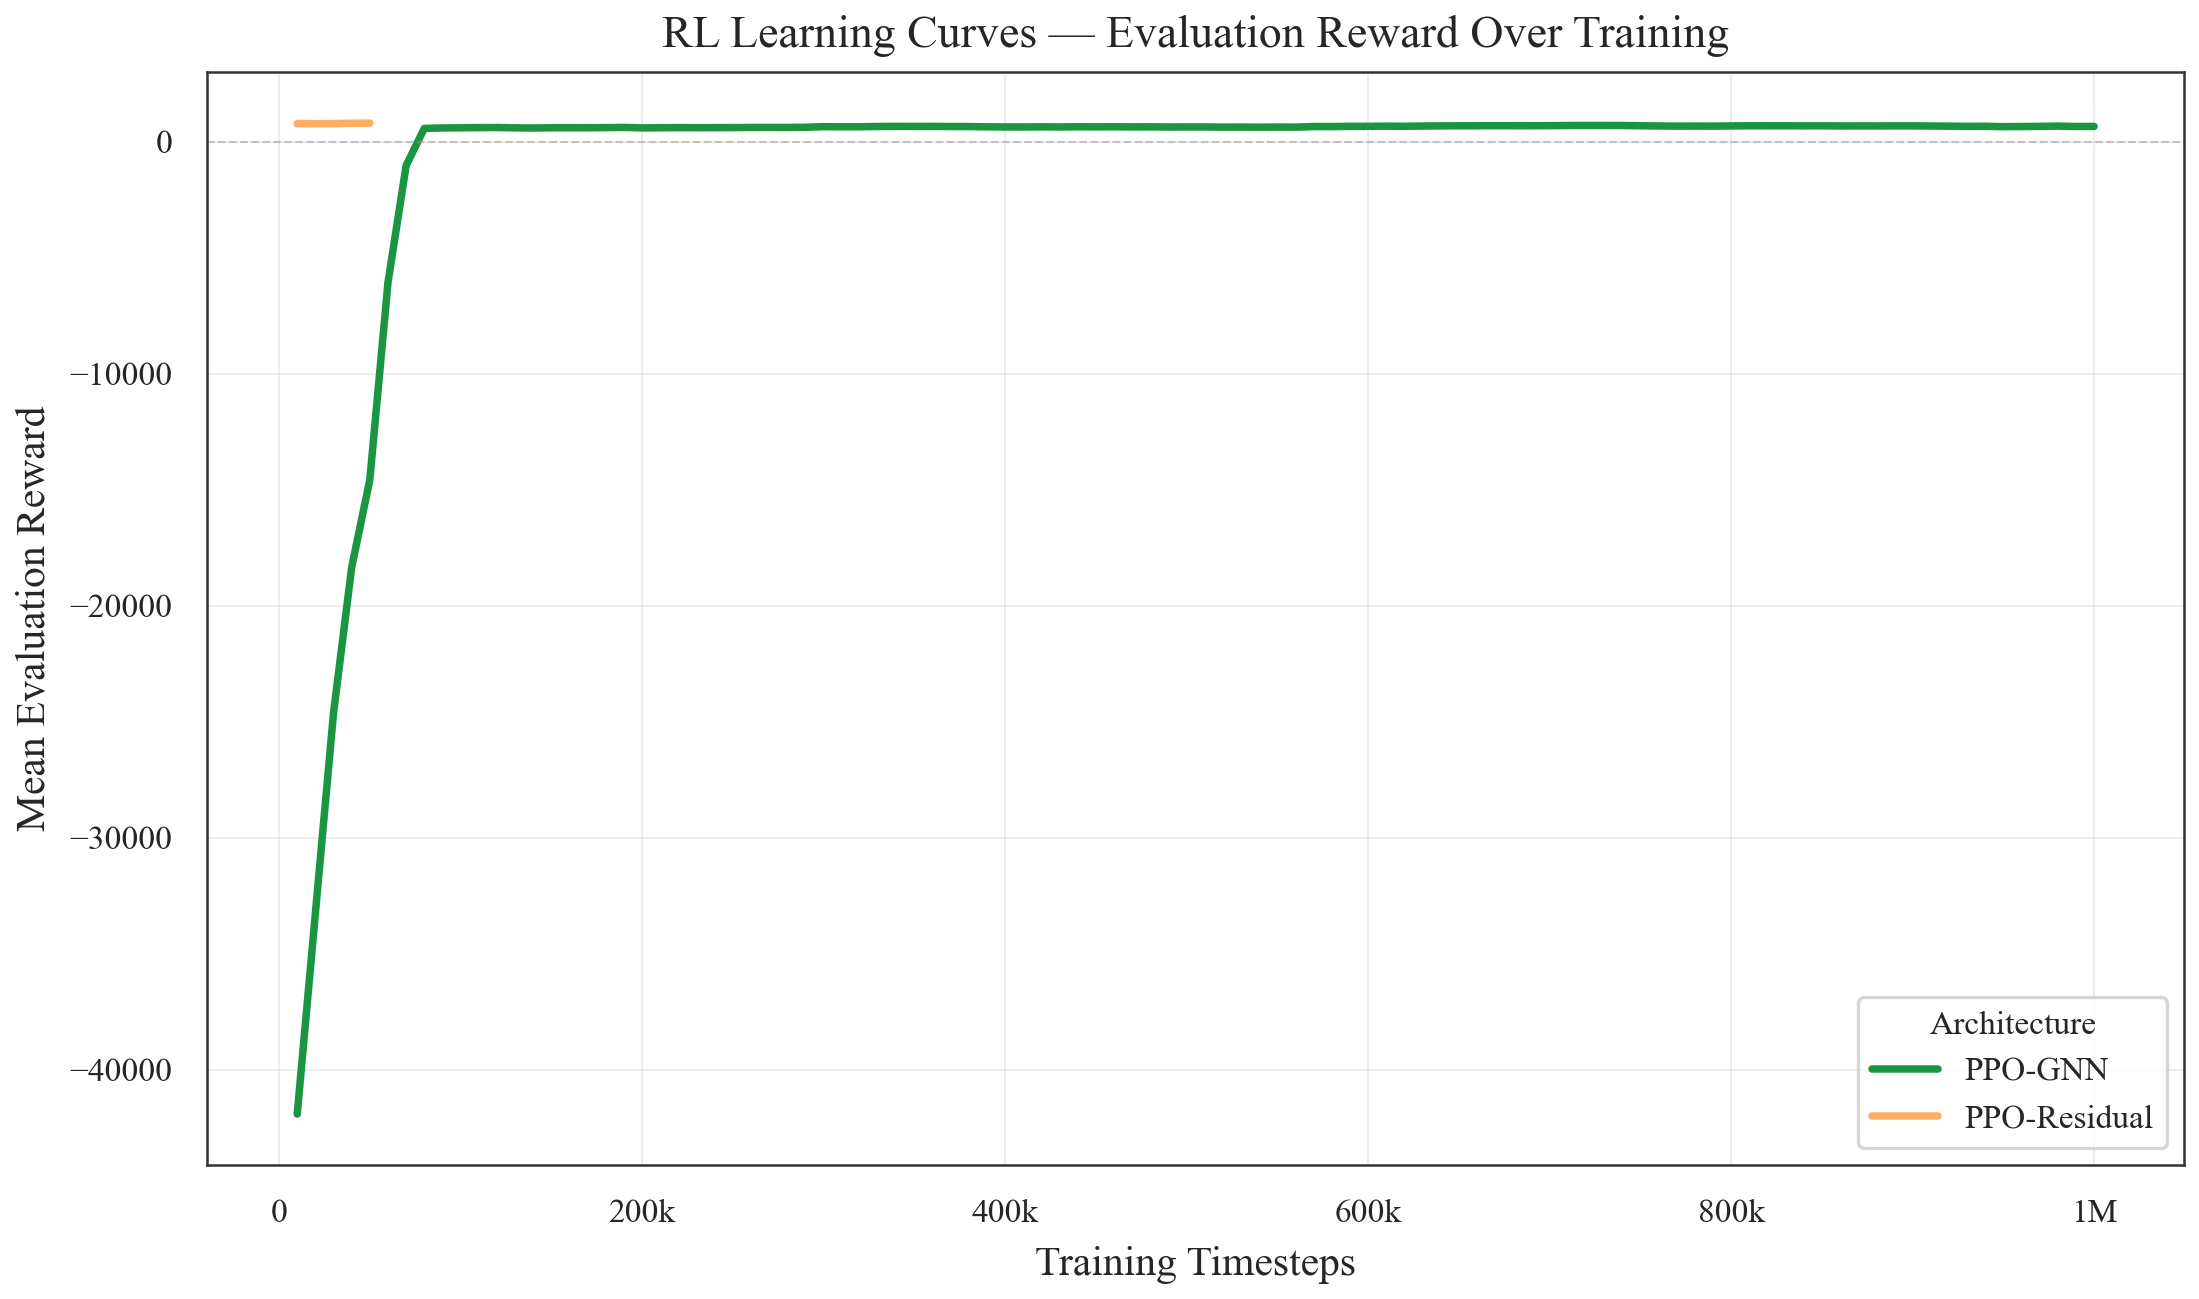
\includegraphics[width=0.58\linewidth]{figures/T1_learning_curves.png}
  \caption[RL training convergence.]{%
    Evaluation reward during training for the two primary RL
    architectures.  PPO-GNN recovers from an initial reward trough
    ($-42$k) within ${\sim}100$k steps; PPO-Residual bootstraps from a
    heuristic base and converges in ${\sim}20$k steps.}
  \label{fig:training_curves}
\end{figure}


\paragraph{A3: Transformer observation-collapse bug (TSPPO).}
The original ``TSPPO'' and ``TSPPO-B'' results in the development
pipeline were generated by a Transformer agent whose
\texttt{get\_action()} method applied \texttt{obs = obs[0]} to a
1-D observation vector, collapsing the entire observation to a single
scalar. The resulting policy was effectively random, yet its
performance (+1{,}052 profit) appeared plausible because the model had
memorised heuristic-like constant actions during training.

This bug was confirmed by two forensic findings:
(i)~TSPPO-B and GNN-V3-B produced \emph{identical} profits across
259/260 episodes (mean $\Delta < 0.75$), indicating both loaded the
same GNN checkpoint due to a path-aliasing error; and
(ii)~the ``TSPPO'' (non-blind) results were also anomalous, showing no
sensitivity to demand type despite the Transformer's spatial-attention
design.

\textbf{Fix:} We retired the contaminated TSPPO/TSPPO-B data,
re-implemented the Transformer agents as \textbf{PPO-Transformer}
(spatial node-token attention) and \textbf{ST-PPO} (spatio-temporal
frame stacking), each with validated observation pipelines and
dimension assertions at agent construction.

\paragraph{A4: GNN extractor wiring mismatch.}
The release-draft training script (\texttt{train\_generalist.py})
imported \texttt{GNNFeatures\allowbreak Extractor} (a plain 2-layer GCN) instead
of the production-grade \texttt{GNNFeatures\allowbreak ExtractorV3} (directed
MPNN with edge features, attention, and residual connections). Legacy
checkpoints, however, had been trained with V3 and contained
pickled module paths (\texttt{src.models.\allowbreak gnn\_extractor\_v3}) that
no longer existed in the release namespace.

\textbf{Fix:} A \texttt{legacy\_shim.py} module was introduced to alias
historical \texttt{sys.modules} paths to the current
\texttt{gym\_invmgmt.extractors.*} namespace, enabling checkpoint
loading without retraining. Behavioral verification against the
historical cache confirmed 3/4 exact profit matches and 1/4 within
2.3\% (a minor floating-point divergence in the lost-sales
fulfillment path).

\paragraph{A5: SAC instability on stationary demand.}
SAC achieves $-13\% \pm 53$ of Oracle on stationary demand despite
using the same observation pipeline as PPO-MLP. Investigation revealed
that the informed SAC training run was highly sensitive to entropy
tuning and serial-topology initialization, producing an unstable final
policy in several stationary rows. The blind variant (SAC-B) performs
substantially better ($61\%$ of Oracle), likely because the reduced
observation dimensionality stabilised the critic's Q-function estimates.
SAC remains in the benchmark as a methodological control for off-policy
vs.\ on-policy comparison rather than as a headline learned-policy
candidate.

%% ================================================================
%%  APPENDIX F — Cross-Study Comparison with Perez et al. (2021)
%% ================================================================
\section{Cross-Study Comparison with Perez et al.\ (2021)}%
\label{sec:perez_comparison}

The \texttt{B\_PaperReplication} block contains stationary
Poisson($\lambda{=}20$), $T{=}30$ evaluations under backlog and
lost-sales fulfillment.  Only the two \emph{base-topology} rows are
used here for comparison with \citet{perez2021}; the serial
rows in the same block are retained for our internal topology axis and
are not Perez replications.  \Cref{tab:perez_comparison} compares the
Table~2 values reported by \citet{perez2021} with the closest
environment-native counterparts in our framework.

This is a cross-study calibration check, not an exact reproduction.
\citet{perez2021} use a different software stack, solver, action
parameterization, RL implementation, sample size, and training budget.
We therefore use the table to verify scale and ordering consistency
and to contextualize the standard PPO baseline, rather than to claim
strict statistical superiority over a prior implementation.  No
conclusion in this appendix relies on the serial, goodwill, M5, or
non-stationary stress-test rows.

\begin{table}[!tbp]
\centering
\caption{Cross-study comparison on the stationary base-topology
benchmark.  ``Perez'' columns reproduce their Table~2 (100 sample
paths, Gurobi~9.1 / Ray~RLlib).  ``Ours'' columns report the
matching base rows from \texttt{B\_PaperReplication} (10 seeds,
PuLP/CBC / SB3).  Our OR entries use informed variants
(MSSP-I/DLP-I) as the closest counterparts to Perez's rolling-horizon
optimizers, which solve with access to the modeled demand process.
\emph{Shaded rows} denote agents unique to our study.}
\label{tab:perez_comparison}
\small
\renewcommand{\arraystretch}{1.05}
\begin{tabular}{@{} l rr c rr @{}}
\toprule
& \multicolumn{2}{c}{\textbf{Perez (2021)}}
& & \multicolumn{2}{c}{\textbf{Ours}} \\
\cmidrule(lr){2-3}\cmidrule(lr){5-6}
\textbf{Agent} & \textbf{Profit} & \textbf{\% Orc}
& & \textbf{Profit} & \textbf{\% Orc} \\
\midrule
\multicolumn{6}{@{}l}{\textit{Backlog mode}} \\
\midrule
Oracle   & 861.3 & 100\%  & & 845.7 & 100\% \\
MSSP-RH / MSSP-I & 802.7 & 93.2\% & & 834.9 & 98.7\% \\
DLP-RH / DLP-I   & 791.6 & 91.9\% & & 804.6 & 95.1\% \\
RL (PPO) & 737.2 & 85.6\% & & ---   & --- \\
\rowcolor{lightgray}
PPO-MLP  & ---   & ---    & & 588.1 & 69.5\% \\
\rowcolor{lightgray}
PPO-GNN (MPNN) & ---   & ---    & & 601.4 & 71.1\% \\
\rowcolor{lightgray}
PPO-Transformer  & ---   & ---    & & 591.3 & 69.9\% \\
\rowcolor{lightgray}
Residual & ---   & ---    & & 766.8 & 90.7\% \\
\midrule
\multicolumn{6}{@{}l}{\textit{Lost-sales mode}} \\
\midrule
Oracle   & 854.9 & 100\%  & & 842.1 & 100\% \\
MSSP-RH / MSSP-I & 790.6 & 92.5\% & & 809.0 & 96.1\% \\
DLP-RH / DLP-I   & 735.8 & 86.1\% & & 755.0 & 89.7\% \\
RL (PPO) & 757.8 & 88.6\% & & ---   & --- \\
\rowcolor{lightgray}
PPO-MLP  & ---   & ---    & & 581.9 & 69.1\% \\
\rowcolor{lightgray}
PPO-GNN (MPNN) & ---   & ---    & & 597.4 & 70.9\% \\
\rowcolor{lightgray}
PPO-Transformer  & ---   & ---    & & 587.0 & 69.7\% \\
\rowcolor{lightgray}
Residual & ---   & ---    & & 762.6 & 90.6\% \\
\bottomrule
\end{tabular}
\end{table}

\Cref{tab:methodology_delta} enumerates the main methodological
differences between the two studies that preclude a direct PPO-vs-PPO
comparison.

\begin{table}[!tbp]
\centering
\caption{Methodological differences between Perez~et~al.\ and our
framework.  These factors confound any direct PPO-vs-PPO comparison
and are deliberate design choices rather than implementation
deficiencies.}
\label{tab:methodology_delta}
\small
\renewcommand{\arraystretch}{1.05}
\begin{tabular}{@{} l l l @{}}
\toprule
\textbf{Dimension} & \textbf{Perez et al.} & \textbf{Ours} \\
\midrule
Action space   & Discrete (enumerated) & Continuous + RescaleAction \\
RL framework   & Ray / RLlib PPO       & Stable-Baselines3 PPO \\
Architecture   & $[256, 256]$ FFN      & $[256, 128]$ MLP \\
Training scope & Specialist (1 per scenario) & Generalist (domain-rand.) \\
Training budget & 70K episodes (${\sim}$2.1M steps) & 500K steps (${\sim}$17K ep.) \\
OR solver      & Gurobi 9.1            & PuLP / CBC \\
Evaluation paths & 100 sample paths & 10 benchmark seeds \\
\bottomrule
\end{tabular}
\end{table}

\paragraph{Key observations.}
\begin{enumerate}[nosep]
\item \textbf{Framework validation via Oracle parity.}
      Our Oracle (+845.7 backlog, +842.1 lost-sales)
      closely matches Perez's (+861.3, +854.9), confirming
      that the environment scale, reward accounting, and stationary
      demand setting are comparable.  The 1.5--1.8\% residual is
      consistent with cross-implementation and sampling differences
      (10 vs.\ 100 sample paths), and is small relative to the
      method-level gaps elsewhere in the benchmark.
\item \textbf{OR solver parity.}
      Our informed rolling-horizon OR baselines are close to, and in
      this stationary slice slightly above, the \citet{perez2021} values:
      MSSP-I reaches 98.7\%/96.1\% of Oracle and DLP-I reaches
      95.1\%/89.7\% in backlog/lost-sales mode.  We do not interpret
      these differences as solver dominance.  They reflect a mixture
      of sample size, implementation details, forecast access, and
      solver stack.  The important shared result is the ordering:
      stochastic rolling-horizon planning outperforms deterministic
      expected-value planning in both studies.
\item \textbf{PPO is a deliberate baseline, not a claimed contribution.}
      The 16--19~pp gap between Perez's specialist PPO
      (85.6\%, 88.6\%) and our generalist PPO-MLP (69.5\%,
      69.1\%) is a cross-study comparison confounded by several
      factors (\Cref{tab:methodology_delta}): continuous vs.\
      discrete action space, smaller training budget, generalist
      vs.\ specialist training scope, framework differences, sample
      size, and network architecture differences.
      Because these factors are entangled, we do not attribute
      the gap to any single cause.
      \emph{We intentionally prioritise generalisation breadth
      over per-scenario peak performance}, as our contribution
      is the comparative framework, not the PPO baseline itself.
\item \textbf{Residual RL recovers OR-level performance.}
      Our Residual agent (90.7\% BL, 90.6\% LS) matches
      Perez's MSSP-RH within 2.5~pp in backlog mode and within
      1.9~pp in lost-sales mode, while also exceeding the Perez PPO
      percentages in this stationary calibration slice.  This supports a cautious
      conclusion: heuristic-anchored residual learning can recover
      much of the performance lost by flat continuous-control PPO in
      this environment-native comparison.  It does not prove that
      Residual RL dominates Perez's specialist PPO under a fully
      matched training protocol; it shows that hybridization is a
      useful design direction when moving from stationary specialist
      experiments to broader generalist benchmarks.
\end{enumerate}

%% ================================================================
%%  APPENDIX G — Scenario-Level Performance Heatmap
%% ================================================================
\section{Scenario-Level Performance Heatmap}\label{sec:appendix_heatmap}

The main manuscript summary tables aggregate performance
across scenario clusters, which can mask important per-scenario
variability. \Cref{fig:scenario_heatmap} therefore presents the
complete, disaggregated performance landscape.

\begin{figure}[p]
  \centering
  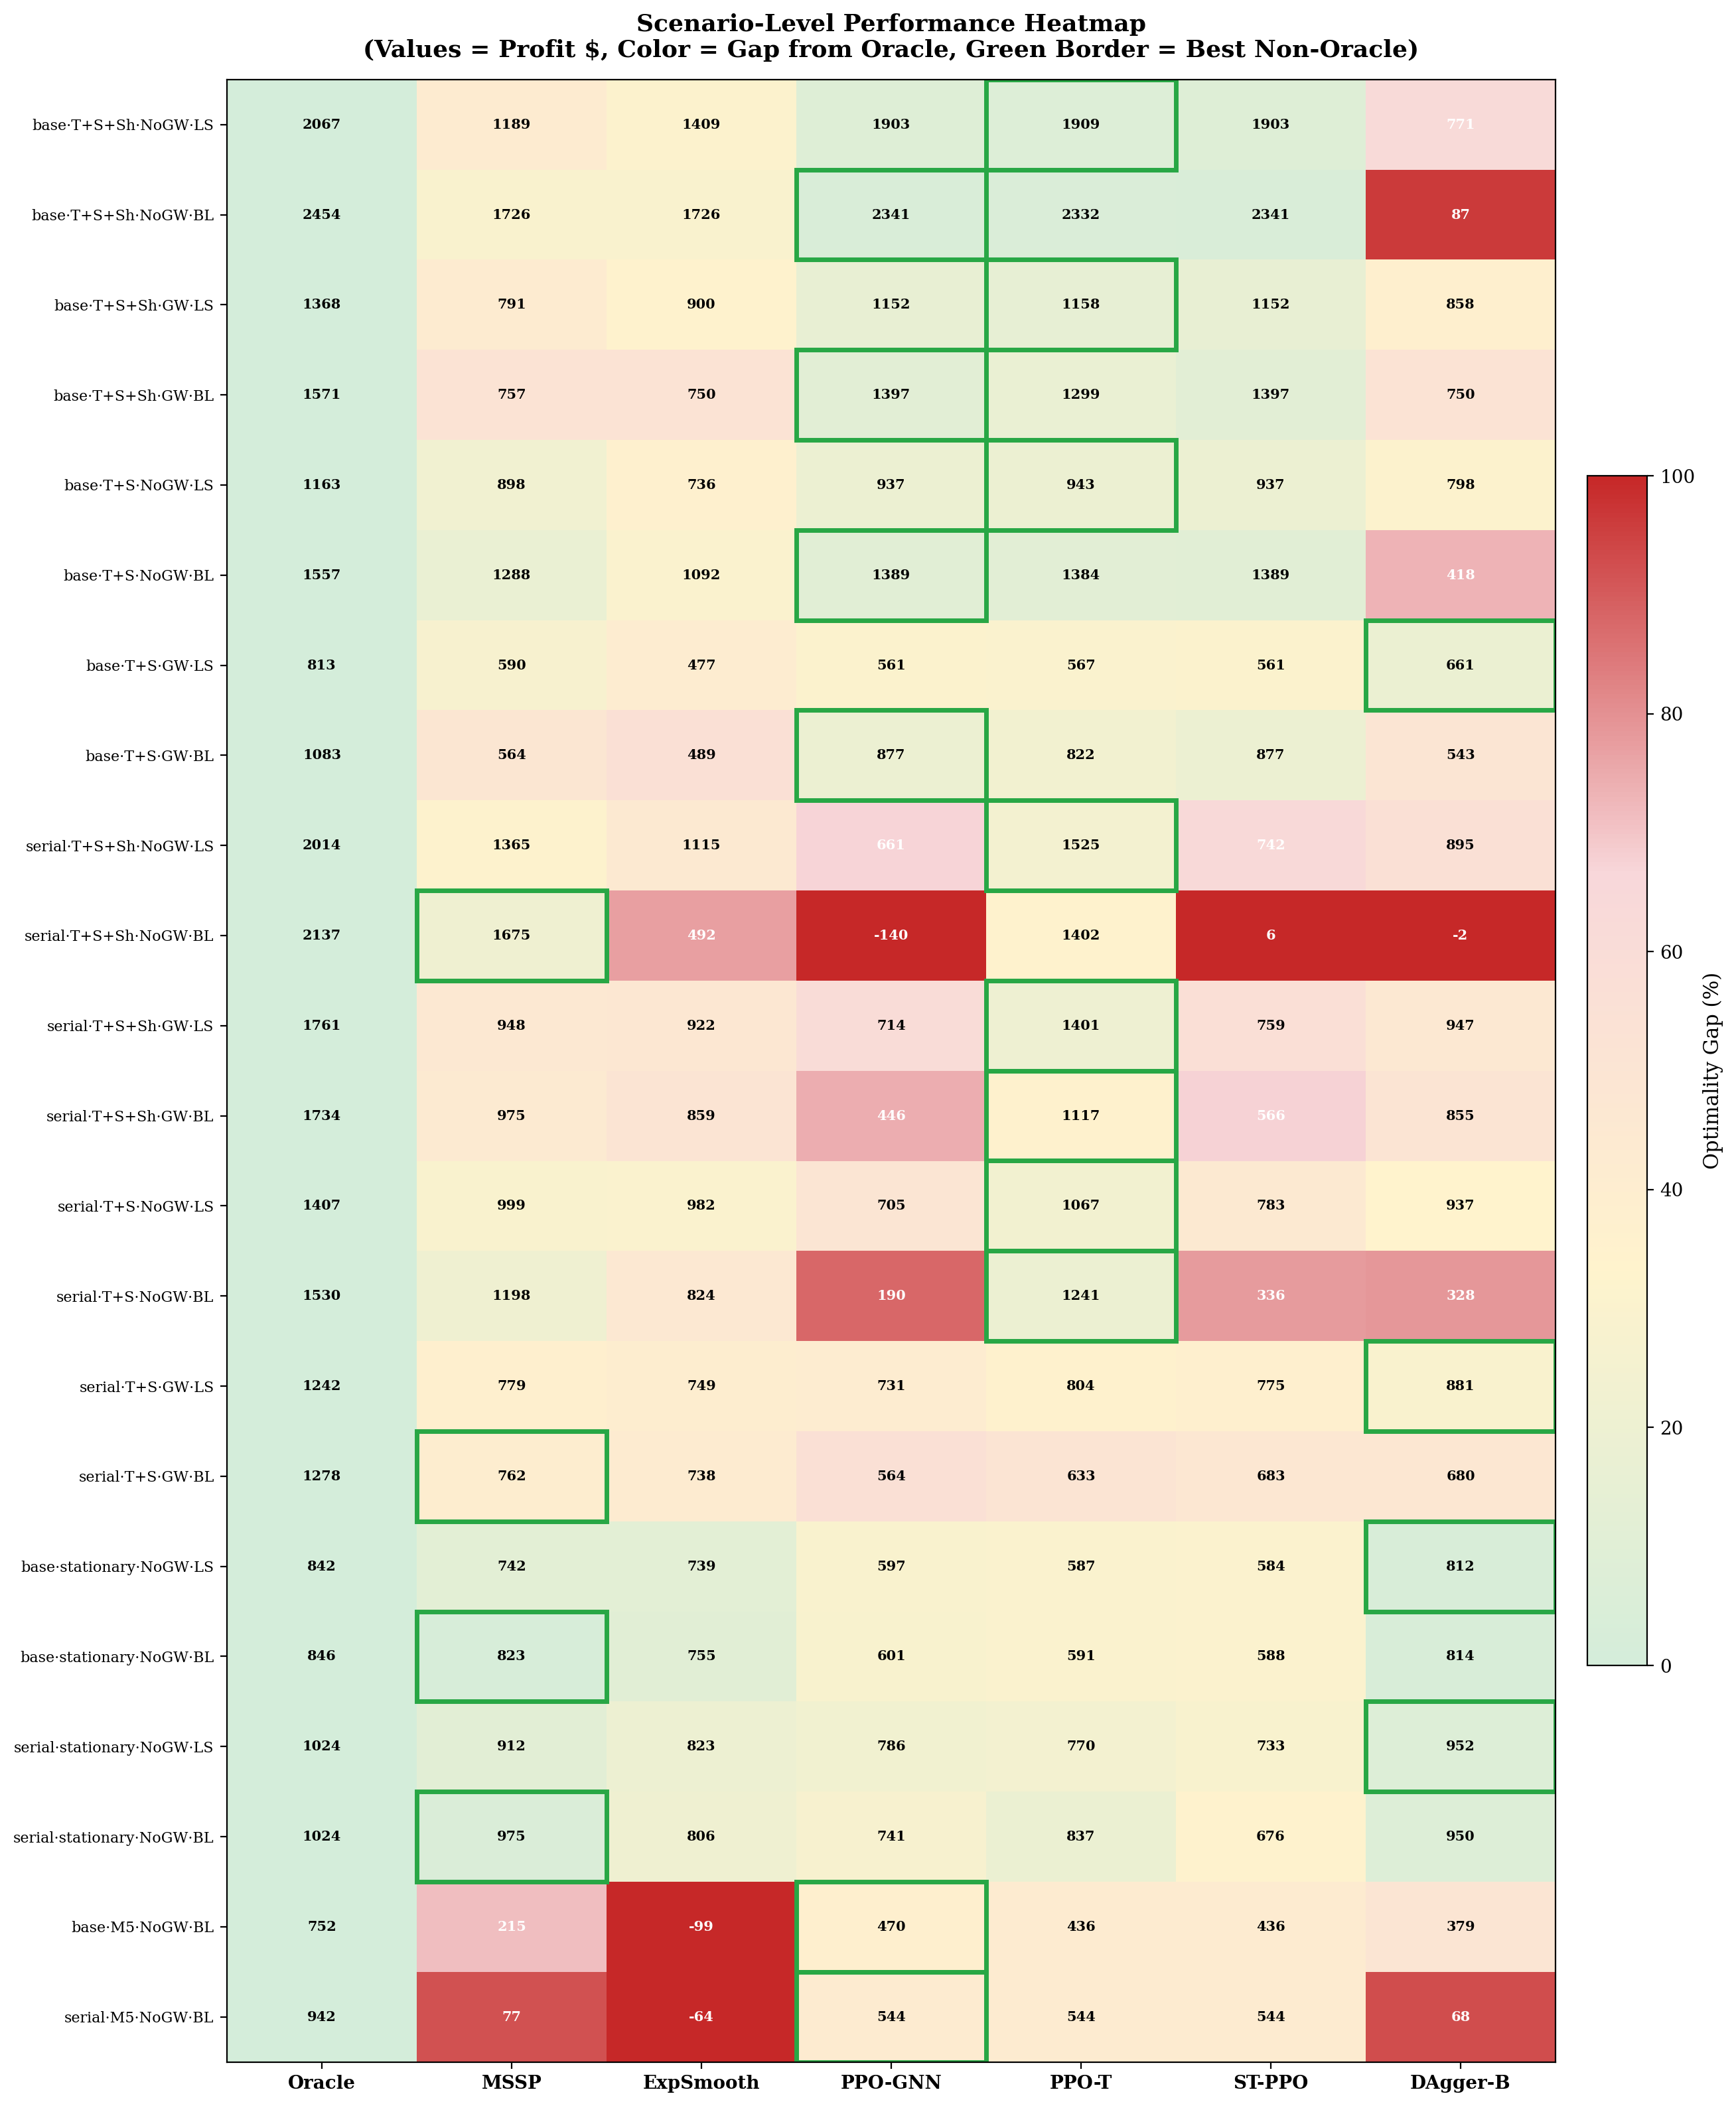
\includegraphics[width=0.82\linewidth,height=0.68\textheight,keepaspectratio]{figures/B1_scenario_heatmap.png}
  \caption[Performance landscape across all 26 scenarios.]{%
    Scenario-level performance heatmap. Cell values are mean
    episodic profit~(\$) over 10 seeded 30-period episodes; color intensity
    encodes the optimality gap from the Oracle upper bound.
    Green borders mark the best non-Oracle agent per row.
    The deepest red cells concentrate in serial-topology
    scenarios with endogenous goodwill.}
  \label{fig:scenario_heatmap}
\end{figure}

Several structural patterns emerge from the heatmap.
\emph{First}, the Oracle upper bound itself varies by more than
$3{\times}$ across scenarios (from about \$752 to \$2,454),
confirming that scenario difficulty is not uniform and
aggregated metrics alone would be misleading.
\emph{Second}, MSSP-I is the dominant non-Oracle method in the current
artifact, achieving the best non-Oracle profit in 24 of 26 scenarios.
The two exceptions are a stationary default lost-sales replication row,
where DAgger-B narrowly leads, and a default topology shock-plus-goodwill
backlog row, where PPO-MLP narrowly leads MSSP-I. Thus, the current
heatmap primarily demonstrates the value of informed scenario hedging,
while still showing that learned policies can be competitive in
particular low-noise or feedback-heavy regimes.
\emph{Third}, wide optimality gaps remain concentrated in serial and
endogenous-goodwill cases for many non-Oracle agents---precisely the
regime where demand erosion and delayed replenishment compound the
credit-assignment problem discussed in the benchmark framework.

%% ================================================================
%%  APPENDIX H — Operational Cost Decomposition
%% ================================================================
\section{Operational Cost Decomposition}\label{sec:appendix_decomposition}

The episodic profit reported in the main manuscript is a single scalar
that aggregates sales revenue and the cost terms defined in the reward
contract defined in the main manuscript. Two agents with identical profits
can achieve them through fundamentally different operational strategies
--- one by maximizing revenue at the expense of high holding costs,
another by minimizing procurement but tolerating stockouts.
This section disaggregates profit into its constituent components
to expose these strategic differences. The decomposition is reported
on the 22 core scenarios used for the main performance averages; the
four supplemental MARL-mode rows are excluded from this appendix table
to keep the operational comparison aligned with the centralized
benchmark narrative.

\Cref{fig:reward_decomp} visualizes three key operational metrics
across agents: total profit, average on-hand inventory, and mean
unfulfilled demand. \Cref{tab:cost_decomposition} provides the
corresponding financial breakdown. Holding combines node on-hand
holding and pipeline holding, while the shortage column corresponds to
the \texttt{BacklogPenalty} KPI column and therefore applies to both
backlog and lost-sales modes.

\paragraph{Key structural insights.}
\begin{enumerate}
  \item \textbf{Blind MSSP misses demand in stress cases.} Even with
    higher average inventory than Oracle (73 vs.\ 59 units), MSSP
    accumulates 847 unfulfilled units and \$85 in shortage penalties,
    compared with Oracle's 231 units and \$23. The failure mode is not
    simply low inventory; it is insufficient hedging and positioning
    under non-stationary demand without informed forecast access.
  \item \textbf{Residual RL over-procures.} Residual achieves high
    revenue (\$3{,}922, exceeding Oracle's \$3{,}731) but pays
    \$2{,}572 in procurement---22\% more than Oracle---because the
    learned residual correction $\delta$ adds a safety buffer atop
    the heuristic baseline.
  \item \textbf{DAgger-B collapses under distribution shift.}
    Its revenue of \$2{,}416 (35\% below Oracle) reveals that
    supervised distillation from the MSSP oracle fails to generalize
    beyond the stationary training distribution, accumulating
    \$160 in shortage penalties---the highest among the selected
    agents in this decomposition.
\end{enumerate}

\begin{figure}[!tbp]
  \centering
  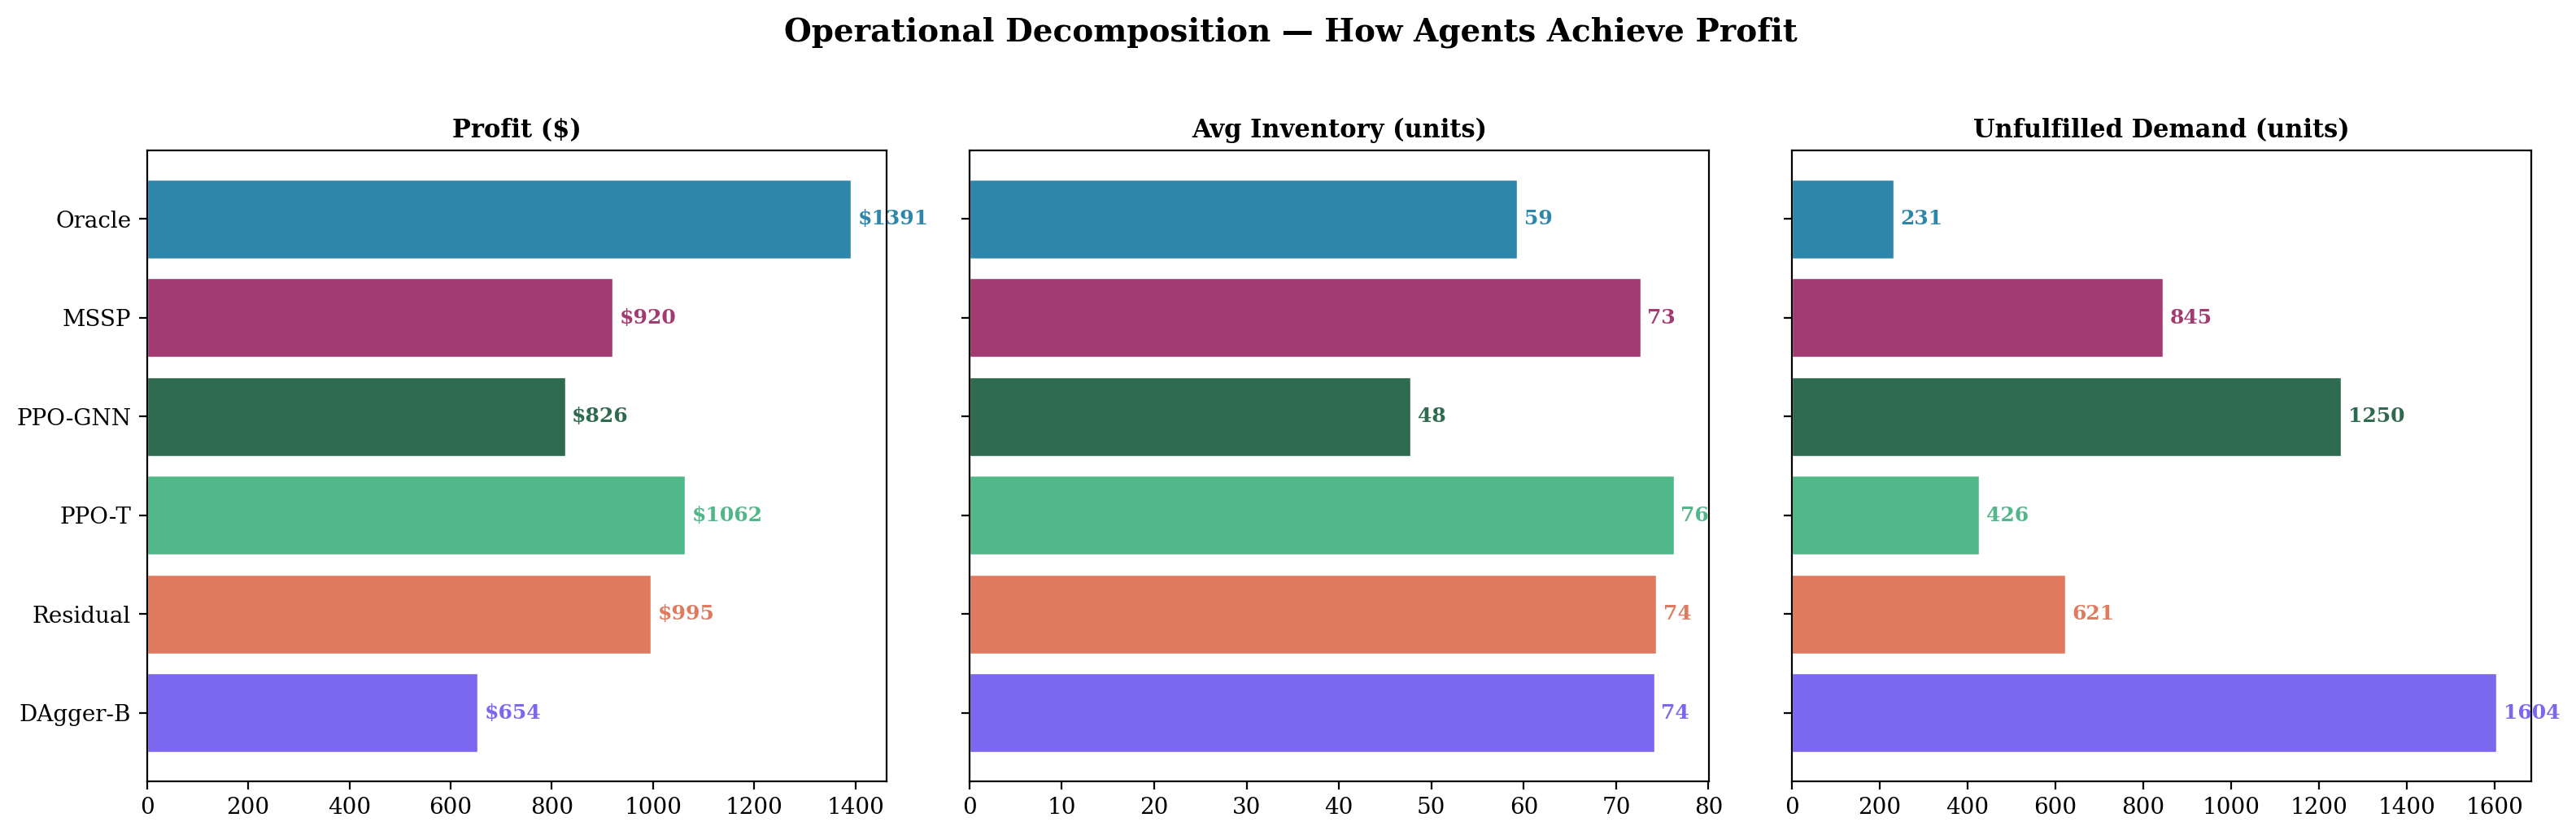
\includegraphics[width=0.85\linewidth]{figures/E4_reward_decomposition.png}
  \caption[Operational decomposition of agent performance.]{%
    Operational decomposition across key agents. \emph{Left:} mean
    episodic profit~(\$). \emph{Center:} average on-hand inventory
    (units). \emph{Right:} mean unfulfilled demand (units). Oracle
    averages 231 units unfulfilled vs.\ MSSP's 847 on the 22 core
    scenarios, explaining the latter's optimality gap despite higher
    average inventory.}
  \label{fig:reward_decomp}
\end{figure}

\begin{table}[!tbp]
\centering
\caption[Mean cost decomposition by agent.]{%
  Mean cost decomposition by agent, aggregated across the 22 core
  scenarios. All values are dollars per 30-period episode. Fixed
  ordering costs are zero in the released scenario matrix and are
  therefore omitted. Data extracted from
  \texttt{benchmark\_final\_merged.csv}.}
\label{tab:cost_decomposition}
\small
\renewcommand{\arraystretch}{1.05}
\begin{tabular}{@{} l r r r r r r @{}}
\toprule
\textbf{Agent} & \textbf{Profit} & \textbf{Revenue} & \textbf{Holding} & \textbf{Shortage} & \textbf{Proc.} & \textbf{Oper.} \\
\midrule
Oracle    & 1{,}391 & 3{,}731 & 194 &  23 & 2{,}113 & 10 \\
MSSP      &   918 & 3{,}018 & 218 &  85 & 1{,}788 & 10 \\
PPO-GNN   &   826 & 3{,}041 & 283 & 125 & 1{,}799 &  8 \\
PPO-MLP   &   833 & 3{,}166 & 297 & 120 & 1{,}908 &  8 \\
PPO-Transformer & 1{,}062 & 4{,}063 & 354 &  43 & 2{,}593 & 11 \\
ST-PPO     &   853 & 3{,}101 & 288 & 112 & 1{,}839 &  8 \\
Residual  &   995 & 3{,}922 & 278 &  62 & 2{,}572 & 15 \\
DAgger-B  &   654 & 2{,}416 & 218 & 160 & 1{,}376 &  8 \\
\bottomrule
\end{tabular}
\end{table}

%% ================================================================
%%  APPENDIX I — Goodwill and Service-Level Diagnostics
%% ================================================================
\section{Goodwill and Service-Level Diagnostics}%
\label{sec:appendix_goodwill}\label{sec:appendix_fill_rate}

A distinguishing feature of \texttt{gym-invmgmt} is its
\emph{endogenous} customer goodwill mechanism defined in the main manuscript,
whereby stockouts erode a sentiment multiplier $s_t$ that directly
scales future demand. The dynamics are deliberately asymmetric:
\begin{equation}
  s_{t+1} = \begin{cases}
    \max(0.2, \; 0.90 \cdot s_t) & \text{if stockout at } t \quad (\text{rapid decay}) \\
    \min(2.0, \; 1.01 \cdot s_t) & \text{otherwise} \quad (\text{slow recovery})
  \end{cases}
\end{equation}
The 10\% decay versus 1\% recovery asymmetry encodes the modeling
assumption that customer trust is lost quickly but rebuilt slowly.
A single stockout reduces the next demand multiplier by 10\%, and
approximately 11 consecutive stockout-free periods are needed to
reverse that one-period decay. In the implementation, a stockout is any
positive unfulfilled quantity on a retail-demand link at the end of a
period.

\Cref{fig:goodwill_impact} compares matched synthetic scenarios with
goodwill off versus on. These bars should be read as a diagnostic of
endogenous demand feedback rather than a fixed-demand treatment effect:
with goodwill enabled, service failures can reduce future market size,
so even the Oracle benchmark faces a different realized demand path.
In the eight goodwill scenarios, MSSP-I remains the strongest causal
non-Oracle benchmark at 89.1\% of Oracle. Among learned policies,
Residual~RL (73.0\%), SAC (72.8\%), and PPO-Transformer (71.4\%)
are the strongest goodwill performers, while blind MSSP falls to
57.9\%. A positive matched-goodwill profit change should not be read
as an unqualified improvement: a weak service policy can sometimes
benefit numerically because prior stockouts shrink later demand and
therefore reduce subsequent fulfillment pressure. The main lesson is
therefore not that goodwill uniformly rewards aggressive ordering, but
that service failures create a path-dependent market-size penalty that
changes the economic value of safety stock and scenario hedging.

\subsection{Service-Level Distributions}

The profit-based metrics in the main manuscript capture economic
performance but obscure an operationally critical dimension:
\emph{service quality}. We report two related but distinct quantities.
The unit-weighted fill rate for agent $a$ in episode $k$ is:
\begin{equation}
  \text{FR}_{a,k}
  =
  \min\left\{1,\;
  \frac{\sum_{t=1}^{T}\sum_{(j,m)\in E_d} S_{a,k,t}^{(j,m)}}
       {\sum_{t=1}^{T}\sum_{(j,m)\in E_d} D_{k,t}^{(j,m)}}\right\}
\end{equation}
where $S_{a,k,t}^{(j,m)}$ is actual retail sales to market node~$m$
and $D_{k,t}^{(j,m)}$ is realized customer demand. The clipping at~1
matches the benchmark implementation and prevents backlog catch-up sales
from producing fill rates above 100\%. The benchmark also records a
stockout-free-period service level:
\begin{equation}
  \text{SL}_{a,k}
  =
  \frac{1}{T}\sum_{t=1}^{T}
  \mathbf{1}\!\left[
    \sum_{(j,m)\in E_d} U_{a,k,t}^{(j,m)} = 0
  \right].
\end{equation}
Thus, a policy can have a high fill rate but a lower service level if it
usually satisfies most units while still stocking out in many periods.
\Cref{fig:fill_rate_dist} plots scenario-level fill-rate means for the
main operational subset used in the decomposition figures. Within this
plotted subset, Oracle is near perfect, PPO-Transformer and Residual
reduce the low-service tail relative to blind MSSP, and PPO-GNN plus
DAgger-B display much wider service-quality dispersion. Across the full
22-scenario core grid, the CSV further shows that MSSP-I substantially
improves mean fill rate over blind MSSP (0.943 vs.\ 0.822), while SAC
matches Oracle's mean fill rate (both 0.949) but at lower profit because
high service can come with excess inventory and procurement cost.

\begin{figure}[!htbp]
  \centering
  \begin{subfigure}[t]{0.48\linewidth}
    \centering
    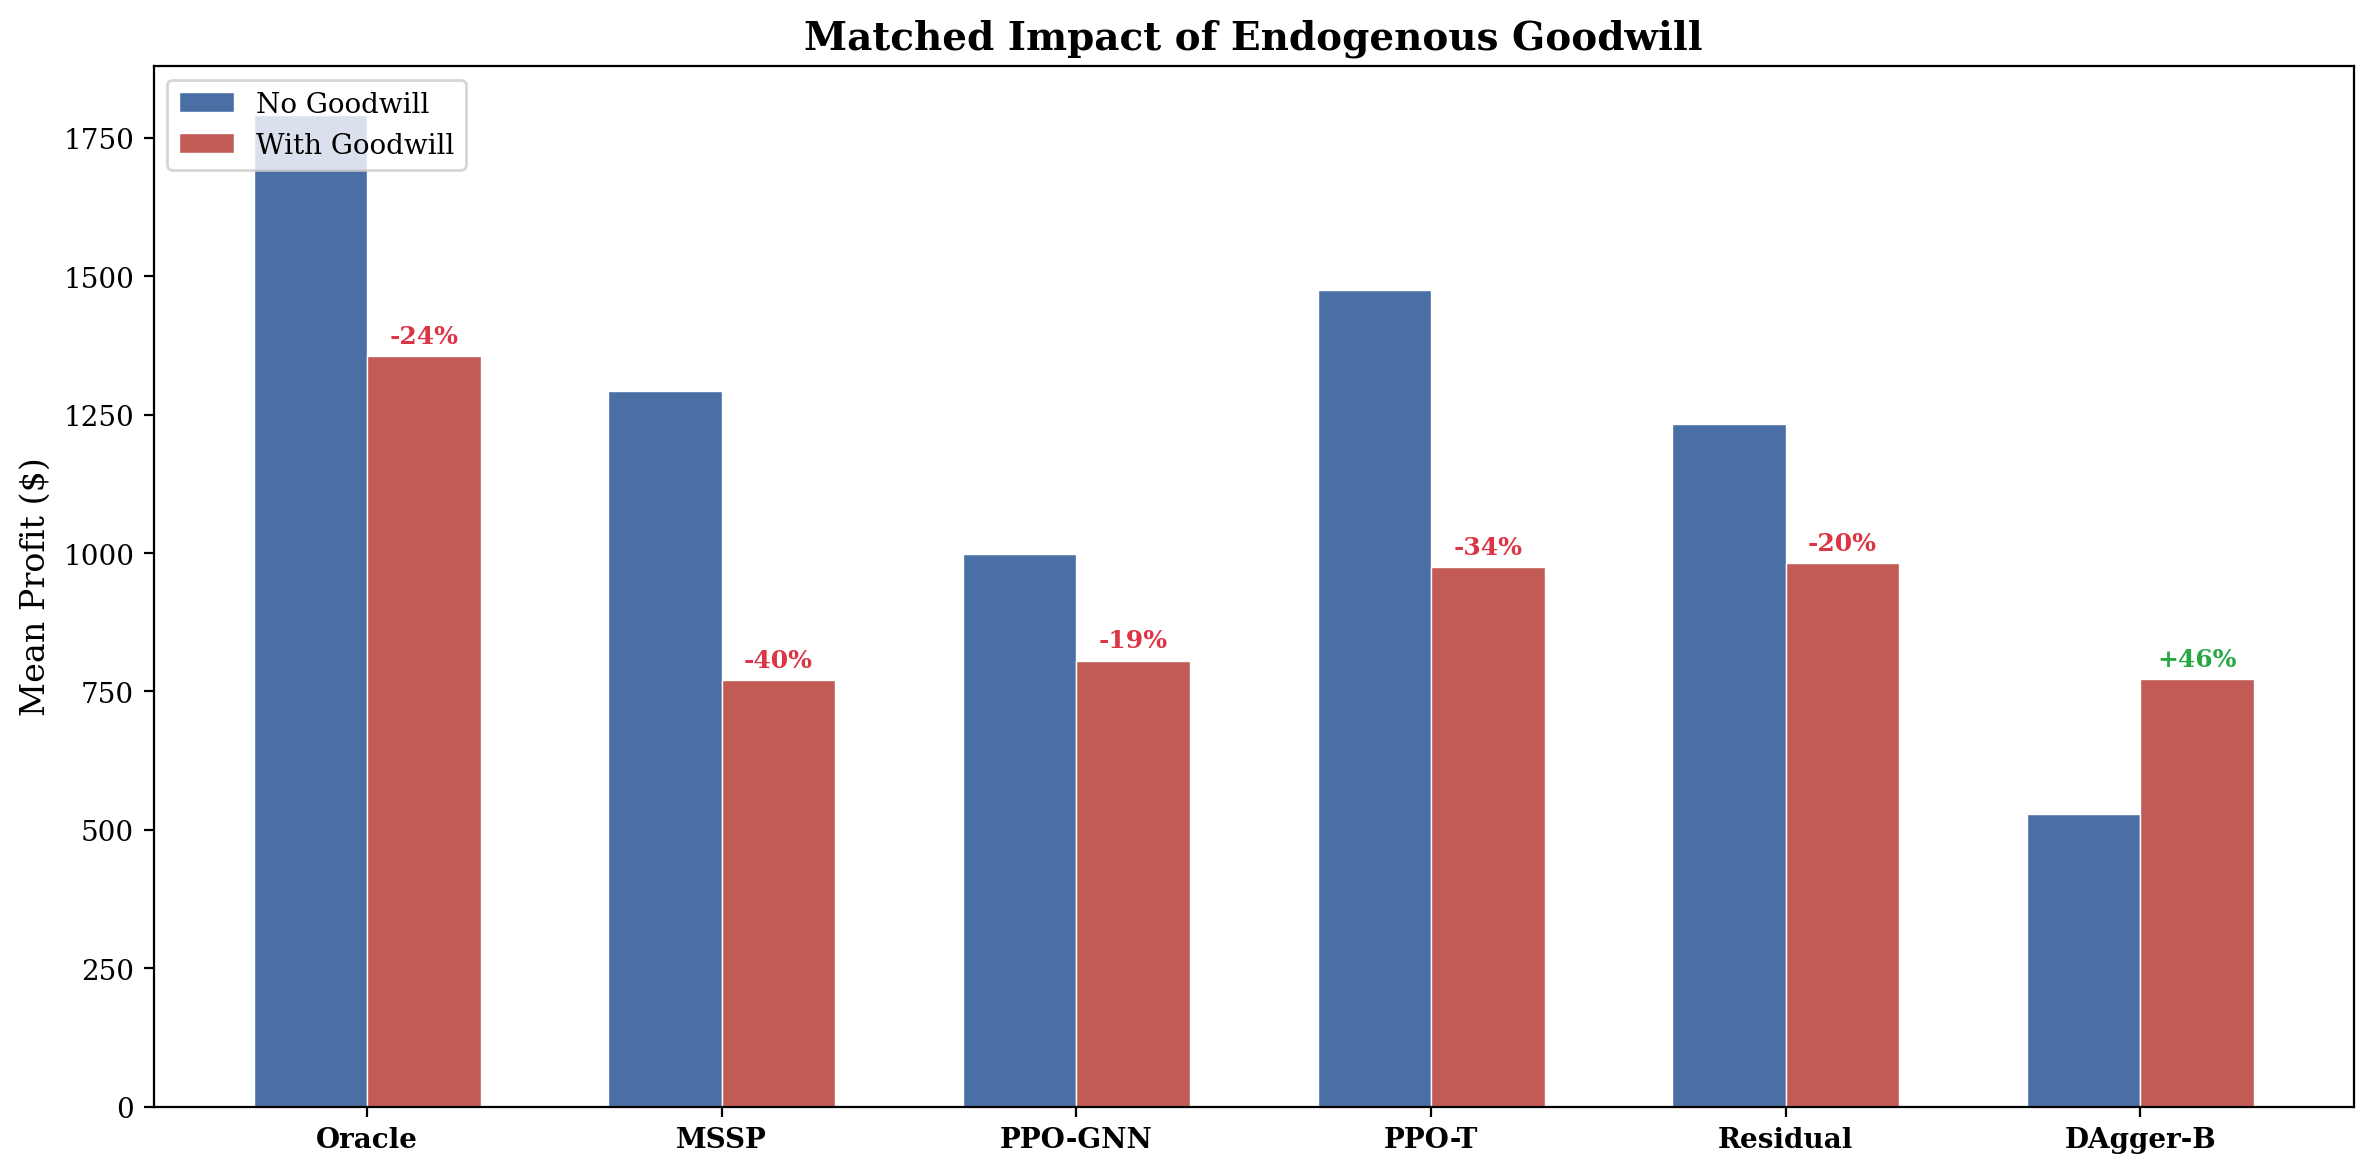
\includegraphics[width=\linewidth]{figures/B3_goodwill_impact.png}
    \caption{Matched-scenario impact of endogenous customer goodwill.
      Paired bars compare matched No-Goodwill vs.\
      With-Goodwill scenarios. Because goodwill changes future demand,
      these bars are diagnostic comparisons rather than fixed-demand
      treatment effects.}
    \label{fig:goodwill_impact}
  \end{subfigure}
  \hfill
  \begin{subfigure}[t]{0.48\linewidth}
    \centering
    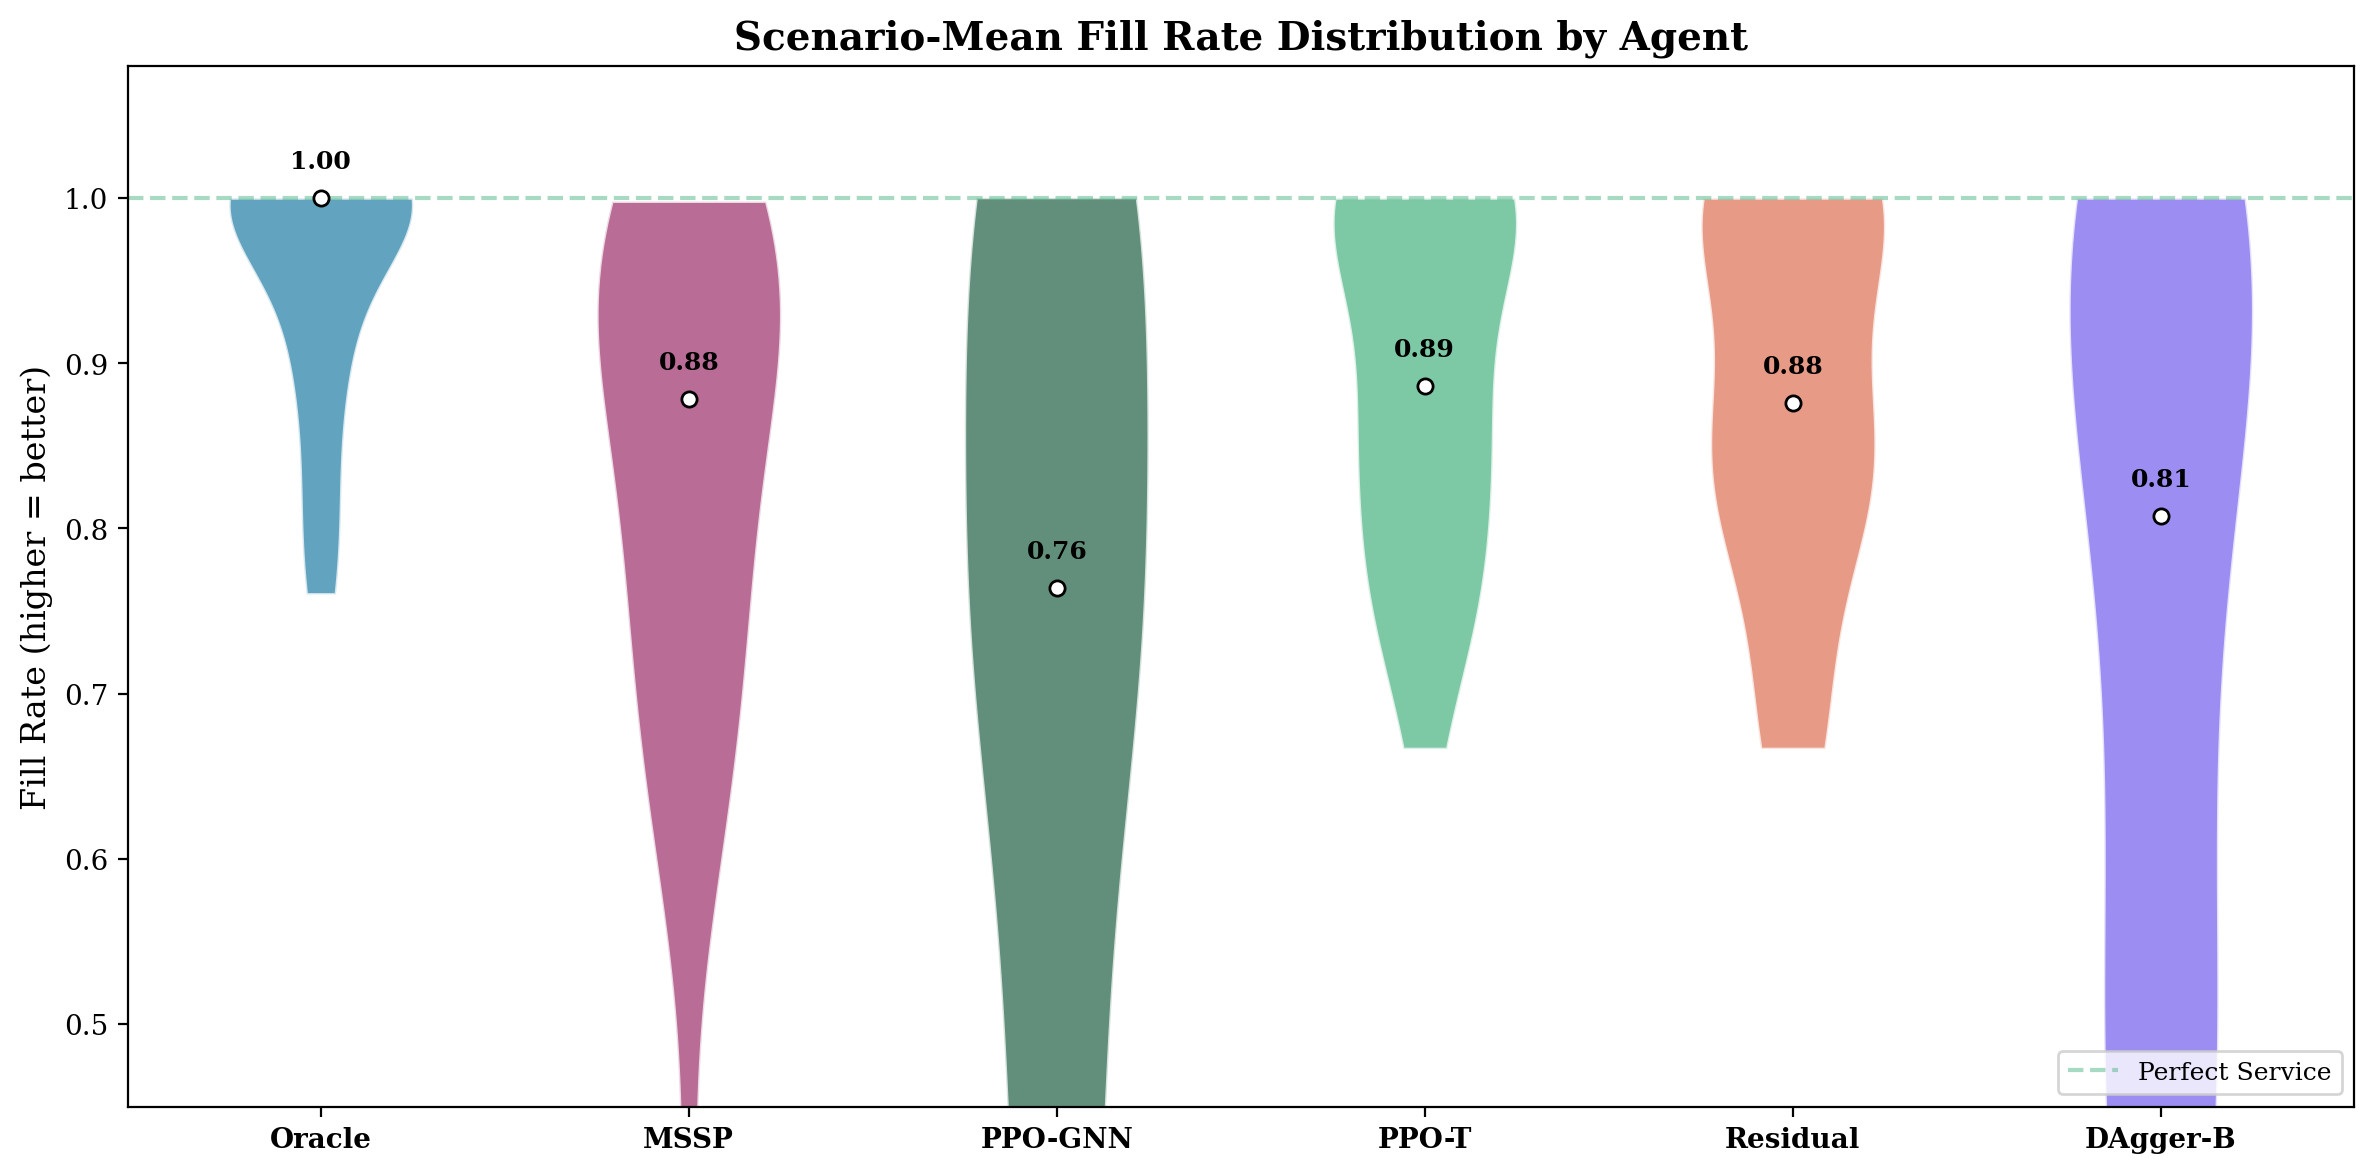
\includegraphics[width=\linewidth]{figures/T4_fill_rate_distribution.png}
    \caption{Fill-rate distributions across scenario-level means.
      Violin widths encode probability density; white dots mark
      medians. PPO-Transformer and Residual substantially reduce the
      low-service tail relative to blind MSSP among the plotted agents.}
    \label{fig:fill_rate_dist}
  \end{subfigure}
  \caption[Service quality analysis: goodwill sensitivity and fill-rate distributions.]{%
    \emph{(a)}~Goodwill sensitivity: percentage annotations show
    matched profit changes when endogenous goodwill is enabled.
    \emph{(b)}~Service-quality consistency: unit-weighted fill rate
    differs from the stockout-free service-level metric reported in
    the benchmark CSV.}
  \label{fig:service_quality}
\end{figure}

%% ================================================================
%%  APPENDIX J — Computational Cost Comparison
%% ================================================================
\section{Computational Cost Comparison}\label{sec:appendix_compute}

A key practical advantage of learned policies over rolling-horizon
mathematical programming is amortization. Once trained, a policy
evaluates a fixed computation graph for the chosen topology and feature
contract; its online cost does not grow with the number of sampled
scenarios in a stochastic program. In contrast, MSSP must solve a new
scenario-tree optimization at every decision epoch, with cost scaling in
the number of scenarios $|\Omega|$, nodes $|V|$, and planning horizon
$T$.

\Cref{tab:compute_times} reports mean wall-clock evaluation times
per 30-period episode over the full 26-scenario merged artifact,
measured on the local Intel Core i5-8257U CPU used for the final audit.
The table uses
\texttt{Time\_Sec} as the canonical timing field produced by the
benchmark runner; auxiliary planning/replay columns are retained in the
CSV for diagnostics but are not mixed into the speed-up calculation.
The fastest heuristic, $(s,S)$-I, is roughly 510$\times$ faster than
blind MSSP, while PPO-MLP and PPO-Transformer are approximately
89$\times$ and 47$\times$ faster, respectively. PPO-GNN is slower than
flat neural policies because it invokes graph feature extraction, while
Residual RL remains fast because its heuristic correction is lightweight
in the released evaluator. LLM-Policy-C is slightly faster than blind
MSSP in the final artifact because it calls the local language model
once per episode rather than once per period, but it remains far slower
than DLP, heuristics, and specialized learned policies.

\Cref{tab:training_times} reports retained one-time training logs for
models retrained during the final audit. These should be read as
hardware-specific provenance records, not universal algorithmic
constants. Some legacy artifacts, including PPO-GNN, Residual, SAC, and
DAgger, are evaluated from shipped checkpoints but are not assigned exact
training-time claims because their original wall-clock logs are not
retained in the release artifact.

% --- Compute Times + Training Times (side-by-side with subcaptions) ---
\begin{table}[!tbp]
\caption[Evaluation and training wall-clock times.]{%
  Computational costs on the local Intel Core i5-8257U CPU used for the
  final audit.}
\label{tab:compute_all}
\scriptsize
\renewcommand{\arraystretch}{1.08}
\centering
\begin{subtable}[t]{0.50\textwidth}
\centering
\caption{Mean evaluation time per episode.}
\label{tab:compute_times}
\begin{tabular}{@{} l r r @{}}
\toprule
\textbf{Agent} & \textbf{Time (s)} & \textbf{Speedup} \\
\midrule
$(s,S)$-I          & 0.021 & 510$\times$ \\
$(s,S)$            & 0.032 & 327$\times$ \\
ExpSmoothing       & 0.036 & 290$\times$ \\
Newsvendor         & 0.049 & 215$\times$ \\
PPO-MLP            & 0.119 & 89$\times$ \\
SAC                & 0.124 & 85$\times$ \\
Residual           & 0.210 & 50$\times$ \\
PPO-Transformer    & 0.223 & 47$\times$ \\
ST-PPO             & 0.258 & 41$\times$ \\
DAgger-B           & 0.261 & 40$\times$ \\
GNN-IL             & 0.266 & 40$\times$ \\
PPO-GNN            & 0.297 & 36$\times$ \\
Oracle$^{\dagger}$ & 0.720 & 15$\times$ \\
DLP-I              & 0.986 & 11$\times$ \\
DLP                & 1.045 & 10$\times$ \\
MSSP-I             & 7.371 & 1.4$\times$ \\
LLM-Policy-C       & 8.998 & 1.2$\times$ \\
MSSP               & 10.575 & 1.0$\times$ \\
\bottomrule
\end{tabular}
\end{subtable}
\hfill
\begin{subtable}[t]{0.46\textwidth}
\centering
\caption{Retained one-time training logs.}
\label{tab:training_times}
\begin{tabular}{@{} l l r @{}}
\toprule
\textbf{Agent} & \textbf{Topology} & \textbf{Time (m)} \\
\midrule
PPO-MLP  & Base           &  17.3 \\
PPO-MLP  & Serial         &  11.7 \\
\rowcolor{lightgray}
PPO-Transformer & Base, Gen.     &  19.6 \\
PPO-Transformer & Serial, Gen.   &  16.2 \\
PPO-Transformer & Base, Blind    &  23.3 \\
PPO-Transformer & Serial, Blind  &  20.2 \\
\rowcolor{lightgray}
ST-PPO    & Base, Gen.     &  79.2 \\
ST-PPO    & Serial, Gen.   &  46.8 \\
ST-PPO    & Base, Blind    & 102.7 \\
ST-PPO    & Serial, Blind  &  82.2 \\
\bottomrule
\end{tabular}
\end{subtable}

\vspace{1mm}
\footnotesize{$^{\dagger}$Oracle timing includes planning plus replay in the benchmark cache. Oracle is a clairvoyant benchmark, not a causal deployable policy, so its timing is reported for reproducibility rather than operational comparison. ``Gen.'' denotes the generalist/informed training contract.}
\end{table}

%% ================================================================
%%  APPENDIX K — Evaluating Foundation Models (LLMs)
%% ================================================================
\section{Evaluating Foundation Models (LLMs)}\label{sec:appendix_llm}

To contextualize our benchmark against prompt-based supply chain agents
such as InvAgent~\citep{quan2024}, we evaluated local foundation-model
controllers using \texttt{Qwen2.5-1.5B-Instruct}~\citep{qwen2024} in GGUF
Q4\_K\_M format with a 4096-token context window. These experiments are
not intended to claim that a 1.5B local model is the strongest possible
LLM controller. Their purpose is narrower: to test whether language
models can be inserted into the same strict action contract as the
other agents and to identify whether failures arise from action
dimensionality, latency, or inventory-cost calibration.

\paragraph{LLM-ZS-Direct (zero-shot raw actions).}
This diagnostic centralized baseline queries the LLM once per period.
Each prompt encodes the current multi-echelon network state as compact
JSON and asks for one reorder quantity per reorder link. The parser
accepts either an ordered list or an \texttt{orders\_by\_link} object,
clips valid quantities to the environment action bounds, and falls back
to a default order vector only if both the original response and one
repair prompt fail.

\paragraph{LLM-Policy-C (centralized parameter policy).}
The full-run LLM baseline uses a more reliable
``LLM-as-strategist, code-as-controller'' design. The LLM is queried
once at the beginning of each episode to select six bounded policy
parameters: \texttt{demand\_multiplier}, \texttt{safety\_z},
\texttt{order\_cap\_fraction}, and tier-specific multipliers for
retail, distribution, and factory nodes. A deterministic graph-aware
base-stock controller then executes those parameters for all 30 periods.
This reduces calls from 30 per episode to one, guarantees a valid action
shape during the episode, and makes the LLM output a strategic prior
rather than a high-frequency actuator.

\paragraph{LLM-InvAgent-C (staged centralized prototype).}
We also implemented an InvAgent-inspired staged centralized prototype
that prompts downstream-to-upstream tiers (retail, distributor, factory)
and passes downstream order signals upstream. This preserves the flavor
of staged supply-chain reasoning, but it is not the full decentralized
multi-agent conversational protocol of InvAgent~\citep{quan2024}. Because
it requires multiple LLM calls per period and was superseded by the
more stable \texttt{LLM-Policy-C} controller, it is retained as an
implementation prototype rather than a headline numerical result in the
canonical merged table.

\paragraph{Evaluation status and results.}
\Cref{tab:llm_diagnostics} summarizes the current LLM evidence. Direct
raw-action prompting was stopped after five completed diagnostic
episodes on the stationary default-topology block because the policy
was already qualitatively dominated: it achieved near-perfect fill rate
by ordering one to two orders of magnitude too much inventory, producing
mean profit of \(-\$52{,}153\), mean inventory above 14{,}000 units,
and mean latency of 439 seconds per episode. Its average parse-failure
rate was 3.3\% of per-period calls, but the larger failure mode was
economic rather than syntactic: valid JSON actions still over-ordered
catastrophically. The bounded policy-parameter variant completed the full
26-scenario/260-episode matrix with zero parse failures. It reaches
60.6\% of Oracle over all 26 scenarios and 59.8\% on the 22-scenario
core grid, with mean fill rate 0.911 and mean stockout-free-period
service level 0.718. Its mean wall-clock latency is 9.0 seconds per
episode, almost all of which is the single initial LLM call.

\begin{table}[!tbp]
\centering
\caption{LLM controller diagnostics. LLM-ZS-Direct is a stopped diagnostic
probe; LLM-Policy-C is the full-run LLM baseline included in the merged
benchmark artifact.}
\label{tab:llm_diagnostics}
\small
\renewcommand{\arraystretch}{1.05}
\begin{tabular}{@{} l l r r r l @{}}
\toprule
\textbf{Variant} & \textbf{Calls} & \textbf{Episodes} & \textbf{Profit} & \textbf{Time (s)} & \textbf{Status} \\
\midrule
LLM-ZS-Direct & 30/episode & 5 & -52{,}153 & 439.1 & stopped diagnostic \\
LLM-Policy-C  & 1/episode  & 260 & 913 & 9.0 & full benchmark \\
LLM-InvAgent-C & multi-call/period & -- & -- & -- & prototype only \\
\bottomrule
\end{tabular}
\end{table}

\paragraph{Interpretation.}
The LLM experiments support a cautious conclusion. Direct raw-action
prompting is not reliable enough for the native inventory-control action
space: even when JSON parsing mostly succeeds, the local model lacks the
cost calibration needed to balance service against holding and
procurement cost. By contrast, policy-level prompting is feasible because
it constrains the LLM to low-dimensional strategic choices and delegates
inventory arithmetic, action dimensionality, and clipping to deterministic
code. The resulting controller is competitive with some simple baselines
but below the strongest heuristic, learned, and OR methods, and it is
slightly faster than blind MSSP but slower than informed MSSP-I and far
slower than fast learned-policy inference in this local setup. We
therefore treat LLMs as strategic policy-parameter generators and
diagnostic baselines, not as drop-in replacements for high-frequency
inventory controllers.

%% ================================================================
%%  APPENDIX L — Empirical Oracle Gap and VSS Analogues
%% ================================================================
\section{Empirical Oracle Gap and VSS Analogues}\label{sec:appendix_vpi}

We report scenario-level empirical gaps between the clairvoyant Oracle
and the rolling-horizon OR baselines, together with benchmark analogues
of the classical \emph{Value of the Stochastic Solution} (VSS) from
stochastic programming~\citep{birge2011}. These statistics are diagnostic
quantities for this benchmark, not theoretical EVPI/VPI estimates. In
particular, MSSP and DLP are finite-horizon rolling approximations, the
MSSP tree uses finite sample-average approximation, and the goodwill
Oracle is a clairvoyant simulation-optimization benchmark rather than a
certified global dynamic-programming optimum.

Here $s$ indexes the 26-row released evaluation artifact (22 core
scenarios plus four supplemental MARL-mode rows), and $\Pi_s^A$ denotes
the seed-averaged episode profit of algorithm $A$ in scenario $s$.

For scenario $s$, the empirical Oracle gaps are:
\begin{equation}
  \Delta^{A}_{s}
  =
  \Pi^{\text{Oracle}}_{s} - \Pi^{A}_{s},
  \qquad A \in \{\text{MSSP},\text{MSSP-I}\}.
\end{equation}
The VSS analogues compare stochastic scenario hedging against the
deterministic expected-value LP under matched information access:
\begin{equation}
  \widehat{\mathrm{VSS}}^{(b)}_{s} =
  \Pi^{\text{MSSP}}_{s} - \Pi^{\text{DLP}}_{s},
  \qquad
  \widehat{\mathrm{VSS}}^{(I)}_{s} =
  \Pi^{\text{MSSP-I}}_{s} - \Pi^{\text{DLP-I}}_{s}.
\end{equation}
We then summarize these 26 scenario-level quantities in
\Cref{tab:vpi_vss}.

\begin{table}[!tbp]
\centering
\caption[Empirical Oracle gaps and VSS analogues.]{%
  Empirical Oracle gaps and VSS analogues across the full 26-row
  released evaluation artifact. Values are dollars per episode, computed
  from scenario-level means over the benchmark seeds.}
\label{tab:vpi_vss}
\small
\renewcommand{\arraystretch}{1.05}
\begin{tabular}{@{} l r r r r @{}}
\toprule
\textbf{Metric} & \textbf{Mean} & \textbf{Std} & \textbf{Min} & \textbf{Max} \\
\midrule
Oracle gap vs. MSSP (\$)      & 469.44 & 255.38 & 22.41  & 864.80  \\
Oracle gap vs. MSSP-I (\$)    &  62.27 &  64.09 &  0.74  & 226.19  \\
VSS analogue, blind (\$)      & 405.58 & 560.41 & -92.71 & 1900.65 \\
VSS analogue, informed (\$)   & 723.18 & 656.02 & 29.63  & 2245.74 \\
\bottomrule
\end{tabular}
\end{table}

The informed stochastic program closes most of the empirical Oracle gap:
the average gap falls from \$469.44 for blind MSSP to \$62.27 for
MSSP-I. This does not mean that MSSP-I is theoretically optimal; it
means that, under the benchmark's finite scenario tree and current
forecast protocol, informed stochastic hedging tracks the clairvoyant
benchmark closely in many scenarios. The VSS analogue is positive for
the informed pair in every scenario (minimum \$29.63), while the blind
analogue is heterogeneous and can be negative when the sampled MSSP tree
hedges too conservatively or reacts poorly to trace-driven demand
relative to the deterministic LP.

%% ================================================================
%%  APPENDIX M — Topology-Transfer Stress Test
%% ================================================================
\section{Topology-Transfer Stress Test}%
\label{sec:appendix_transfer}

The main benchmark trains and evaluates topology-matched checkpoints
for the base and serial topologies.  This appendix reports a separate
\emph{diagnostic stress test}, outside the canonical 26-scenario CSV:
can a graph residual policy trained on one topology be executed
zero-shot on structurally different graphs?  Because the ladder is
small and hand-designed, it probes transfer failure modes rather than
estimating population-level topology generalization.  It should not be
interpreted as evidence that topology-invariant inventory control is
solved.

The transfer policy is a transfer-specific \textbf{Residual GCN-Pool}
controller trained for 200{,}000 timesteps on L0, the 9-node divergent
topology.  The implementation uses graph-only observations, an explicit
heuristic-action observation tail for the residual anchor, and a
per-edge actor that can emit an action vector matching the current
topology.  These design choices remove fixed action-vector
incompatibility, but they do not guarantee that learned edge scores
remain operationally calibrated under different lead-time, cost, and
flow structures.  We therefore evaluate both profit and operational
service KPIs.

\subsection{Transfer Ladder and Protocol}

The hand-designed transfer ladder contains five topologies:
\begin{enumerate}[itemsep=2pt]
  \item \textbf{L0~Divergent (9 nodes).}  Training topology:
    2~raw material suppliers, 3~factories, 2~distributors, and
    1~retailer with multi-path allocation and heterogeneous lead times.
  \item \textbf{L1~Reduced Divergent (7 nodes).}  A pruned variant
    that removes one raw-material source and one factory while
    preserving the broad divergent motif.
  \item \textbf{L2~Diamond (5 nodes).}  A symmetric diamond graph with
    balanced bifurcation and reconvergence.
  \item \textbf{L3~Extended Serial (6 nodes).}  A serial chain with a
    dual-source upstream segment, introducing a bottleneck absent from
    the training topology.
  \item \textbf{L4~Serial (5 nodes).}  A minimal linear chain, maximally
    different from the multi-path divergent training graph.
\end{enumerate}

The ladder is intended to span common structural motifs rather than a
statistically representative sample of supply chains.  For each
topology, the transfer policy and a topology-aware Newsvendor heuristic
reference are evaluated over $n=20$ seeded episodes.  Welch tests and
standardized effect sizes compare profit distributions within each
topology.  These tests quantify whether the heuristic--policy gap is
reliable; they are not used to claim that the transferred policy is
operationally adequate.

\subsection{Reward Transfer}

\Cref{tab:transfer_full} summarizes the retained reward-level results
for these custom topologies, which are reported separately rather than
merged into \texttt{benchmark\_final\_merged.csv}.  The transferred
policy remains profitable on all tested graphs and retains
41.8--84.3\% of the Newsvendor heuristic's profit.  The gap to the
heuristic is statistically significant in every row, so the result is
best read as \emph{partial reward transfer}, not parity with a
topology-aware heuristic.

\begin{table*}[!htbp]
\centering
\caption[Zero-shot topology-transfer reward summary.]{%
  Zero-shot topology-transfer reward summary.  The Residual GCN-Pool
  policy is trained on L0~Divergent and evaluated without fine-tuning on
  all rows.  $\bigstar$ marks the training topology.  Values are dollars
  per 30-period episode over 20 seeds.}
\label{tab:transfer_full}
\small
\renewcommand{\arraystretch}{1.05}
\resizebox{\linewidth}{!}{%
\begin{tabular}{@{} l l rr rr rr rr r @{}}
\toprule
& &
  \multicolumn{2}{c}{\textbf{Newsvendor}} &
  \multicolumn{2}{c}{\textbf{Resid.\ GCN}} &
  \multicolumn{2}{c}{\textbf{95\% CI (GCN)}} &
  \multicolumn{2}{c}{\textbf{Gap Test}} & \\
\cmidrule(lr){3-4} \cmidrule(lr){5-6} \cmidrule(lr){7-8} \cmidrule(lr){9-10}
\textbf{Level} & \textbf{Topology}
  & Mean & Std
  & Mean & Std
  & Lower & Upper
  & $p$ (Welch) & $d$
  & \textbf{\% H} \\
\midrule
\rowcolor{lightgray}
L0 $\bigstar$ & Divergent (9)
  & 782 & 47 & 479 & 41 & 460 & 499
  & $7.3{\times}10^{-23}$ & 6.89 & 61.3\% \\
L1 & Reduced (7)
  & 856 & 48 & 601 & 41 & 582 & 620
  & $5.3{\times}10^{-20}$ & 5.75 & 70.1\% \\
\rowcolor{lightgray}
L2 & Diamond (5)
  & 1330 & 52 & 1121 & 38 & 1103 & 1139
  & $3.2{\times}10^{-16}$ & 4.55 & 84.3\% \\
L3 & Ext.\ Serial (6)
  & 998 & 23 & 417 & 30 & 403 & 431
  & $4.1{\times}10^{-39}$ & 21.62 & 41.8\% \\
\rowcolor{lightgray}
L4 & Serial (5)
  & 833 & 23 & 443 & 30 & 429 & 458
  & $4.8{\times}10^{-33}$ & 14.46 & 53.3\% \\
\bottomrule
\end{tabular}%
}
\end{table*}

\Cref{fig:transfer_gradient} visualizes the same pattern: profit
retention is highest on the symmetric diamond graph and weakest on the
extended serial graph. The non-monotonic ladder suggests that transfer
difficulty is not only a function of node count; bottlenecks, lead-time
placement, and edge semantics matter.

\begin{center}
  \centering
  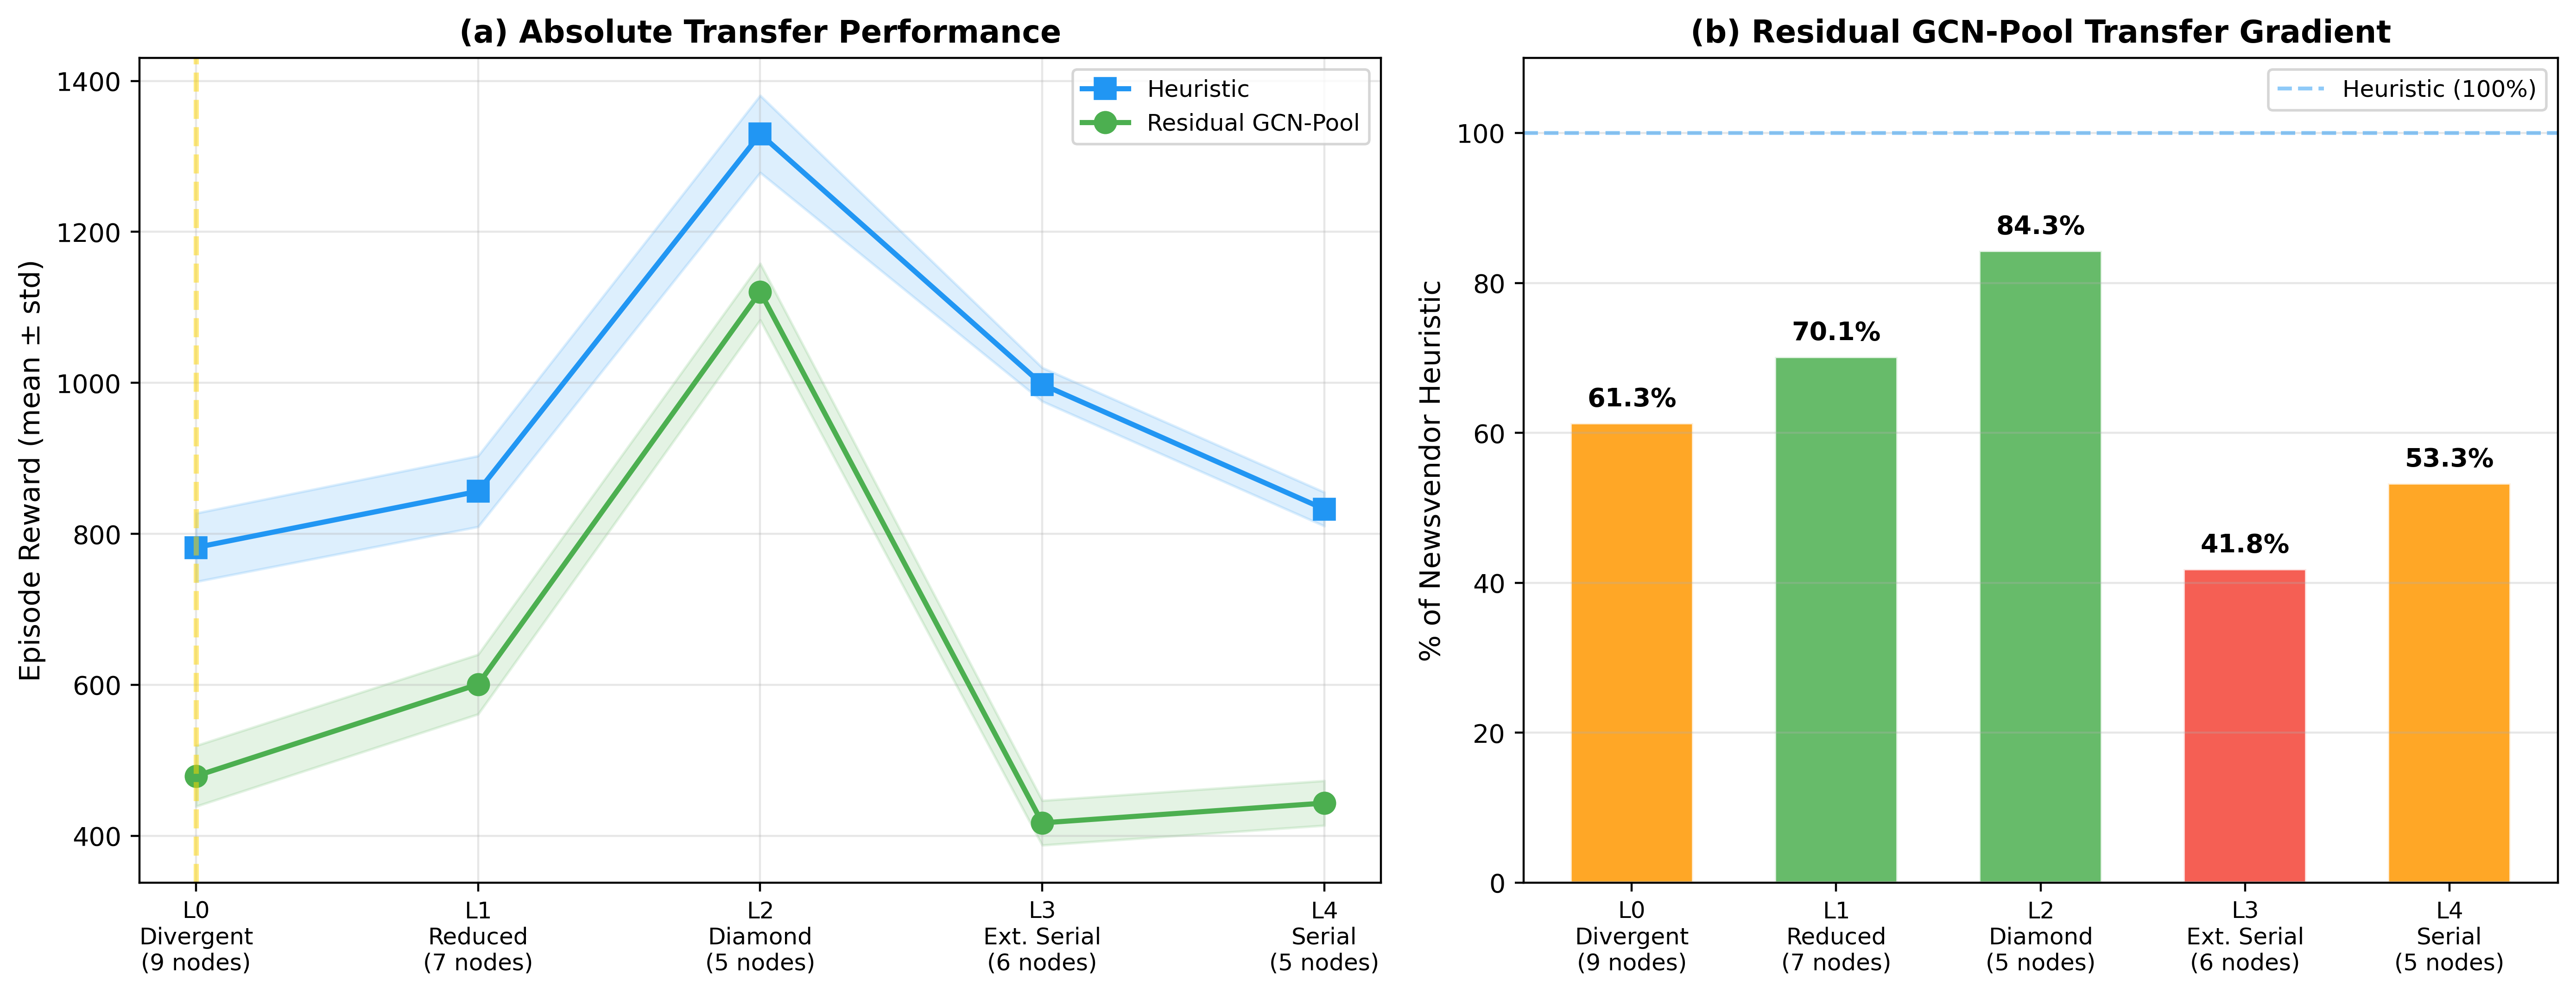
\includegraphics[width=0.84\linewidth]{figures/transfer_gradient.png}
  \captionof{figure}[Zero-shot transfer gradient across five topologies.]{%
    Zero-shot transfer gradient of the Residual GCN-Pool stress-test
    policy. \emph{(a)}~Absolute reward with $\pm 1\sigma$ bands.
    \emph{(b)}~Percentage of Newsvendor heuristic profit retained per
    topology.}
  \label{fig:transfer_gradient}
\end{center}

\subsection{Operational Failure Mode}

Profit alone hides the most important transfer failure.
\Cref{tab:transfer_kpis} decomposes the same experiment using fill
rate, average inventory, holding cost, and backlog penalty.  Fill rate
is computed as total units sold divided by total customer demand.

\begin{table}[!htbp]
\centering
\caption[Operational KPI decomposition for topology transfer.]{%
  Operational KPI decomposition for the zero-shot transfer stress test.
  Holding and backlog-penalty values are mean totals per 30-period episode.}
\label{tab:transfer_kpis}
\small
\renewcommand{\arraystretch}{1.05}
\begin{tabular}{@{} l rr rr rr rr @{}}
\toprule
& \multicolumn{2}{c}{\textbf{Fill Rate (\%)}}
& \multicolumn{2}{c}{\textbf{Avg Inventory}}
& \multicolumn{2}{c}{\textbf{Holding (\$)}}
& \multicolumn{2}{c}{\textbf{Backlog (\$)}} \\
\cmidrule(lr){2-3} \cmidrule(lr){4-5} \cmidrule(lr){6-7} \cmidrule(lr){8-9}
\textbf{Topology} & Heur. & GCN & Heur. & GCN & Heur. & GCN & Heur. & GCN \\
\midrule
\rowcolor{lightgray}
Divergent (9) $\bigstar$
  & 98.1 &  0.0 &  766 &  947 &  259 & 303 &    24 & 1{,}983 \\
Reduced (7)
  & 98.1 &  0.0 &  508 &  583 &  171 & 195 &    17 & 1{,}544 \\
\rowcolor{lightgray}
Diamond (5)
  & 100.0 & 0.0 &  335 &  365 &  122 & 110 &     0 & 1{,}983 \\
Ext.\ Serial (6)
  & 71.8 &  0.0 &  144 &  220 &   60 &  80 &   366 & 5{,}723 \\
\rowcolor{lightgray}
Serial (5)
  & 34.7 &  0.0 &   91 &  129 &   43 &  53 &   865 & 5{,}727 \\
\bottomrule
\end{tabular}
\end{table}

The transfer policy earns positive profit but records zero retail fill
rate in the retained run.  This profitability--service dissociation is
not acceptable as an inventory-control policy.  It indicates that the
graph encoder and residual mechanism preserve some reward-relevant
structure, while the downstream ordering semantics fail to route stock
to the customer-facing link.  The serial topologies make the failure
most visible: backlog penalties rise above \$5{,}700 per episode for
the transfer policy, compared with \$366--\$865 for the heuristic.

\subsection{Interpretation and Limits}

The safe conclusion is modest: graph policies can execute across
topologies and retain some reward signal, but reliable service requires
topology-calibrated edge decoding, lead-time-aware embeddings, explicit
retail-service objectives, and, likely, few-shot target calibration.

\FloatBarrier
\begingroup
\small
\bibliographystyle{plainnat}
\bibliography{references}
\endgroup

\end{document}
